%% Copernicus Publications Manuscript Preparation Template for LaTeX Submissions
%% ---------------------------------
%% This template should be used for copernicus.cls
%% The class file and some style files are bundled in the Copernicus Latex Package, which can be downloaded from the different journal webpages.
%% For further assistance please contact Copernicus Publications at: production@copernicus.org
%% https://publications.copernicus.org/for_authors/manuscript_preparation.html


%% Please use the following documentclass and journal abbreviations for preprints and final revised papers.

%% 2-column papers and preprints
\documentclass[journal abbreviation, manuscript]{copernicus}



%% Journal abbreviations (please use the same for preprints and final revised papers)


% Advances in Geosciences (adgeo)
% Advances in Radio Science (ars)
% Advances in Science and Research (asr)
% Advances in Statistical Climatology, Meteorology and Oceanography (ascmo)
% Aerosol Research (ar)
% Annales Geophysicae (angeo)
% Archives Animal Breeding (aab)
% Atmospheric Chemistry and Physics (acp)
% Atmospheric Measurement Techniques (amt)
% Biogeosciences (bg)
% Climate of the Past (cp)
% DEUQUA Special Publications (deuquasp)
% Earth Surface Dynamics (esurf)
% Earth System Dynamics (esd)
% Earth System Science Data (essd)
% E&G Quaternary Science Journal (egqsj)
% EGUsphere (egusphere) | This is only for EGUsphere preprints submitted without relation to an EGU journal.
% Earth Observation (eo)
% European Journal of Mineralogy (ejm)
% Geochronology (gchron)
% Geographica Helvetica (gh)
% Geoscience Communication (gc)
% Geoscientific Instrumentation, Methods and Data Systems (gi)
% Geoscientific Model Development (gmd)
% History of Geo- and Space Sciences (hgss)
% Hydrology and Earth System Sciences (hess)
% Journal of Bone and Joint Infection (jbji)
% Journal of Environmentally Compatible Air Transport System (jecats)
% Journal of Micropalaeontology (jm)
% Journal of Sensors and Sensor Systems (jsss)
% Magnetic Resonance (mr)
% Mechanical Sciences (ms)
% Natural Hazards and Earth System Sciences (nhess)
% Nonlinear Processes in Geophysics (npg)
% Ocean Science (os)
% Polarforschung - Journal of the German Society for Polar Research (polf)
% Proceedings of the International Association of Hydrological Sciences (piahs)
% Proceedings of the International Ocean Drilling Programme (piodp)
% Safety of Nuclear Waste Disposal (sand)
% Scientific Drilling (sd)
% SOIL (soil)
% Solid Earth (se)
% State of the Planet (sp)
% The Cryosphere (tc)
% Weather and Climate Dynamics (wcd)
% Web Ecology (we)
% Wind Energy Science (wes)


%% \usepackage commands included in the copernicus.cls:
%\usepackage[german, english]{babel}
%\usepackage{tabularx}
%\usepackage{cancel}
%\usepackage{multirow}
%\usepackage{supertabular}
%\usepackage{algorithmic}
%\usepackage{algorithm}
%\usepackage{amsthm}
%\usepackage{float}
%\usepackage{subfig}
%\usepackage{rotating}
%==============================================================
%  notation.tex  —  shared math notation for InSAR / SWE papers
%  Usage: put \input{notation} in the preamble of every paper.
%  Edit a definition here once and it updates in all manuscripts.
%==============================================================

%--- Core quantities ------------------------------------------
\newcommand{\swe}{\mathrm{SWE}}        % was \mathrm{SWE} (x12)
\newcommand{\dswe}{\Delta\swe}         % SWE change: unifies \Delta\mathrm{SWE} and stray \triangle
\newcommand{\dphi}{\Delta\phi}         % interferometric phase change (x10)
\newcommand{\phizero}{\phi_{0}}        % scene-wide reference offset
\newcommand{\rmse}{\mathrm{RMSE}}      % RMSE in math mode
\newcommand{\rsq}{r^{2}}               % r-squared (use $\rsq$ in prose too)

%--- Roman subscripts (one helper, consistent everywhere) -----
\newcommand{\rsub}[1]{_{\mathrm{#1}}}  % generic roman subscript
\newcommand{\ssnow}{\rsub{snow}}         % external dataset
\newcommand{\sext}{\rsub{ext}}         % external dataset
\newcommand{\ssar}{\rsub{SAR}}         % SAR-measured
\newcommand{\scoh}{\rsub{coh}}         % decorrelation / coherence
\newcommand{\strue}{\rsub{true}}       % true value
\newcommand{\snonsnow}{_{\mathrm{non\text{-}snow}}} % fixes the non-snow / non\text{-}snow split

%--- Composite terms you reuse --------------------------------
\newcommand{\dphisar}{\dphi\ssar}      % \Delta\phi_{SAR}
\newcommand{\dphiext}{\dphi\sext}      % \Delta\phi_{ext}
\newcommand{\dphiswe}{\dphi\rsub{SWE}} % \Delta\phi_{SWE}

%--- Draft annotation (grep out [[ ]] before submitting) ------
\usepackage{xcolor}
\newcommand{\note}[1]{\textcolor{red}{[[#1]]}}



\begin{document}

\title{Snow accumulation variability limits InSAR SWE retrieval}


% \Author[affil]{given_name}{surname}

\Author[1][zmhoppinen@alaska.edu]{Zachary}{Hoppinen} %% correspondence author
\Author[1]{Simon}{Zwieback}
\Author[2]{Ross}{Palomaki}
\Author[3]{Hans-Peter}{Marshall}

\affil[1]{Geophysical Institute, University of Alaska Fairbanks, 2156 Koyukuk Drive, Fairbanks, AK}

% \affil[1]{Institute of Arctic and Alpine Research, University of Colorado, 4001 Discovery Dr, Boulder, CO 80303, USA}
\affil[2]{Institute of Arctic and Alpine Research, University of Colorado, 4001 Discovery Dr, Boulder, CO 80303, USA}
\affil[3]{Department of Geosciences, Boise State University, 1910 University Drive, Boise, ID 83725, USA}

%% The [] brackets identify the author with the corresponding affiliation. 1, 2, 3, etc. should be inserted.

%% If an author is deceased, please add \deceased[$Deceased date if applicable$]{$Author number$} (e.g. \deceased[13 November 2015]{2}) at the end of the affiliations. The author number depends on the placement of the author in the author list, e.g. the third author has number 3.


%% If authors contributed equally, please add \equalcontrib{$Author numbers$} (e.g. \equalcontrib{1,3}) at the end of the affiliations. The author number depends on the placement of the author in the author list, e.g. the third author has number 3.




\runningtitle{Snow accumulation variability limits InSAR SWE retrieval}
\runningauthor{Z. Hoppinen et al.}




\received{}
\pubdiscuss{} %% only important for two-stage journals
\revised{}
\accepted{}
\published{}

%% These dates will be inserted by Copernicus Publications during the typesetting process.


\firstpage{1}

\maketitle



\begin{abstract}
Repeat-pass interferometric Synthetic Aperture Radar (InSAR) can retrieve changes in snow water equivalent ($\dswe$) from the phase delay of radar waves through new snow, but typical interferogram processing averages the phase over windows of tens of meters and assumes the $\dswe$ signal is stationary within them. We tested this assumption with four pairs of repeat airborne-lidar snow surveys over the Tuolumne basin and a NISAR acquisition triplet. The lidar-derived $\dswe$ power spectrum breaks at a consistent 27~m (IQR 22--31~m) length scale, so the field varies strongly within an 80~m multi-look window, and the stationarity assumption fails. We capture the resulting effects in a complex sub-window factor $M$. The variance within the window shortens $M$ and decreases coherence, and the skew within the window rotates $M$ and biases the recovered phase from the mean $\dswe$ phase. At L-band, this $\dswe$ variability within the window alone lowers the basin-median coherence to 0.25--0.47, before any temporal or thermal decorrelation, while the retrieval bias causes at most millimeters of SWE error in windows that pass a coherence mask. The two NISAR pairs, one spanning a storm and one during a no-accumulation period, show coherence at 20 and 80~m pixel sizes consistent in space and time with these predictions. The effect of sub-window variability is frequency-dependent, lowering the higher frequency C-band coherence factor to a median of 0.10 while leaving the lower frequency P-band nearly unaffected (0.88). Because the decorrelation grows with the multi-look footprint size, processing interferograms finer than NISAR's standard 80~m posting recovers much of the L-band coherence loss, and a 20~m footprint nearly doubles the median coherence factor. Sub-window $\dswe$ variability is, therefore, a sampling limit that can be predicted from high-resolution snow measurements and used to guide the choice of multi-look footprint for SWE retrievals.
\end{abstract}


% \copyrightstatement{TEXT} %% This section is optional and can be used for copyright transfers.


\introduction  %% \introduction[modified heading if necessary]
Snow water equivalent (SWE), the water stored within a snowpack, is a primary input for water supply forecasting, reservoir management, and flood mitigation in snow-fed basins. No current method provides accurate, consistently available, and spatially distributed SWE estimates over watershed scales in complex terrain. Interferometric Synthetic Aperture Radar (InSAR) is a developing tool for measuring SWE that has the potential to provide large-scale, approximately weekly observations of SWE change ($\dswe$). Recent studies using tower \citep{Leinss2015, Ruiz2021}, airborne \citep{Marshall2021, Nagler2022, Tarricone2023, Hoppinen2023w2, palomaki2025spatiotemporal-df9, Bonnell2024}, and satellite \citep{Belinska2022, Oveisgharan2024, ruiz2024} datasets have shown promising initial results. The newly launched NASA-ISRO SAR (NISAR) mission now provides the systematic, frequent L-band coverage these retrievals require, delivered as standard 80~m geocoded unwrapped interferogram (GUNW) products. Whether that posting adequately samples the snow signal at L-band is still unclear.

The proposed $\dswe$ retrieval from InSAR uses the fact that electromagnetic waves move slower through snow than through air \citep{Guneriussen2001, Leinss2015}. This means that if there is an increase in snow between two acquisitions, the two-way travel time of the electromagnetic waves between the sensor and the ground increases. This causes a phase change between the acquisitions, proportional to the change in snow. The direct equation requires an estimate of snow density, but several approximations have been proposed that directly relate $\dswe$ to phase change ($\dphi$) as a function of local incidence angle ($\theta$) and the central SAR wavelength ($\lambda$) \citep{Leinss2015, Oveisgharan2023}. These approximations can be generalized to a single factor $\kappa(\theta,\lambda)$ relating the phase change to the SWE change:

\begin{equation}\label{eq:dswe2dphi}
    \dphi = \kappa (\theta, \lambda) \dswe
\end{equation}

\noindent which is inverted to retrieve $\dswe$ from an observed $\dphi$.

While past retrieval studies have shown promising results, whether the $\dswe$ signal is adequately sampled by current InSAR techniques has not been quantified directly from the snow field itself. Answering this requires quantifying how $\dswe$ varies in space. To our knowledge, this has not been done because the necessary repeat snow surveys have only recently become available. Past work shows that depth and SWE vary rapidly over short distances (tens of meters) and more gradually over longer distances (hundreds of meters). This is framed as two regimes that each scale consistently with distance, with a decrease in the rate of variation between the short and long length scales. \citep{deems2006, trujillo2007topographic-0ec, Clark2011, mendoza2020, Miller2022}. These studies either operate on snow depth directly ($H\ssnow$) or estimate snow density to derive SWE ($\rm SWE = \frac{\rho\ssnow}{\rho\rsub{water}} H\ssnow$). These prior works measure the snowpack present at one time, depth directly, or SWE via an estimated density, not its change between two acquisitions. This static SWE already varies considerably near the InSAR resolution scale, so the $\dswe$ between two passes may vary as much and complicate sampling the snow signal.

InSAR struggles to sample a signal whose phase changes too quickly across the averaged window. The principle that a geophysical signal varying within the resolution cell degrades the interferogram is well established for ground deformation. \citet{Massonnet1998} defines the maximum detectable InSAR gradient as one fringe, one cycle ($2\pi$) of phase change, over a range change of one pixel, beyond which the fringes lose coherence, and states that when averaging ``several adjacent pixels to form a larger pixel, these limits become more stringent''. The non-stationarity of the $\dswe$ signal explored here is the snow analog of this deformation gradient, with one addition: a deformation gradient is a smooth, symmetric ramp that only decreases the observed coherence, whereas a skewed sub-window $\dswe$ distribution could also bias the recovered multi-looked phase.

Two previous works have inferred sub-window $\dswe$ phase variability from the interferograms themselves. \citet{LiSturm2002} shows that a spatial variation in new-snow accumulation of $>11$~cm (assuming a density of 0.3~g cm$^{-3}$) or redistribution into dunes of half this height across a window can cause decorrelation of C-band interferograms. They then show that mapped patterns of coherence loss from ERS-1 interferograms over the Alaskan arctic slope aligned with the timing and spatial patterns of wind-driven snow redistribution. \citet{ming2026} decomposes the observed coherence over first-year sea ice into volumetric, thermal, baseline, and phase contributions. They note that their phase-coherence term arises from this sub-window $\dswe$ variability within the multi-looking window. 

Our work extends these studies in three ways. To understand how true $\dswe$ variability affects the observed phase and coherence in InSAR $\dswe$ retrievals, we use pairs of co-registered lidar snow depth surveys over the Tuolumne watershed to estimate spatially distributed $\dswe$ and predict the resulting within-window coherence loss. We test these predictions against Tuolumne NISAR coherence maps from snowy and non-snowy periods across a range of multi-looking resolutions. We further show that, due to the wrapped complex nature of the observed phase, a skewed within-window $\dswe$ distribution biases the recovered phase and thus the retrieved SWE. Finally, we use the same lidar fields to measure the power spectrum of $\dswe$ and identify the length scales where these sub-window effects occur.

\section{Theoretical framework}\label{sec:theoretical-framework}

The basis for multi-looking, or performing a complex average of phase over a spatial window, is that it provides a reasonable estimate of what would be measured if many independent observations of the phase could be obtained from the same place and time. This averaging reduces phase noise from random scatterers and improves the estimate of coherence \citep{Bamler1998}. However, this estimate is only valid under the assumption of stationarity: that every pixel in the window samples the same underlying distribution, with the same mean and variance of phase. This assumption is violated when the true $\dswe$ varies across the multi-look window.

To show this effect, we first model the phase $\phi (x)$ of each single-look-complex (SLC) resolution cell $x$ within a spatial multi-look window as the phase of the window-mean $\dswe$ ($\bar{\phi}$) plus a per-cell deviation $\delta (x)$. To simplify notation, we use $\phi = \dphi$ for the remainder of this section, and discussions about phase refer to the change in phase between two observations at the same location at different points in time.

\begin{equation}\label{eq:sigma_def}
      \phi (x) = \underbrace{\bar{\phi}}_{\substack{\text{phase of} \\ \text{mean $\dswe$}}}
           + \underbrace{\delta (x)}_{\substack{\text{per-cell deviation} \\ \text{from mean}}}
\end{equation}

\noindent The observed complex value for the window, assuming unit amplitude in each cell, is:

\begin{equation}\label{eq:z_window}
    \bar{z}\rsub{window}
      = \frac{1}{N} \sum_{x=1}^{N} e^{i\phi(x)}
      \equiv M e^{i\bar{\phi}}
\end{equation}

\noindent where $e^{i\bar{\phi}}$ carries the phase of the window-mean $\dswe$, and $M$ is a complex factor whose magnitude reflects the spread of the per-cell deviations and whose argument captures the retrieval bias relative to the phase of the window-mean $\dswe$.

\begin{equation}\label{eq:def_m}
    M = \frac{1}{N} \sum_{x=1}^{N} e^{i\delta(x)}
\end{equation}

Because $\delta$ is the deviation from the window mean, it has a zero mean by construction. Stationarity makes its variance spatially constant. Under the stationarity assumption, the SWE phase is also the same across the window, so $\delta$ is decorrelation noise alone. For distributed scatterers, this noise is symmetric about the mean and approximately Gaussian at usable coherence. The magnitude $|M|$ is set by the variance of these decorrelation induced deviations and results in the observed decorrelation. The symmetry makes the expected $M$ real-valued, so $\arg(M)=0$ and the expected retrieval bias is zero.

However, when cells within the window are drawn from different distributions, $M$ neither leaves the mean phase unbiased nor converges to the ensemble coherence. $\dswe$ variation across the window centers the per-cell phase distributions on different values, decreasing the length of $M$ and dropping the estimated coherence below the ensemble value. If the within-window $\dswe$ distribution is asymmetric, $M$ also acquires a nonzero argument, rotating the multi-looked phase from the expected phase of the mean $\dswe$ \citep{fischer1993}.

Figure~\ref{fig:theoretical_example} shows three idealized cases, with all other decorrelation sources removed, to isolate the effect of in-window $\dswe$ variability. The three panels differ only in the within-window distribution of $\dswe$. Multi-looking assumes that the samples in the window share a single phase, so the constant case (left) is the only one that meets this condition. Its variance sets the length of the resultant $∣M∣$ as the phase values from each sample of $\dswe$ vary (middle and right). Its skew sets its rotation $\arg(M)$ as the asymmetric circular distribution rotates the recovered window phase from the phase of the window-mean $\dswe$ (right). Here, we treat all per-cell amplitudes as one, though real backscatter amplitudes vary across the window.

\begin{figure}
    \centering
    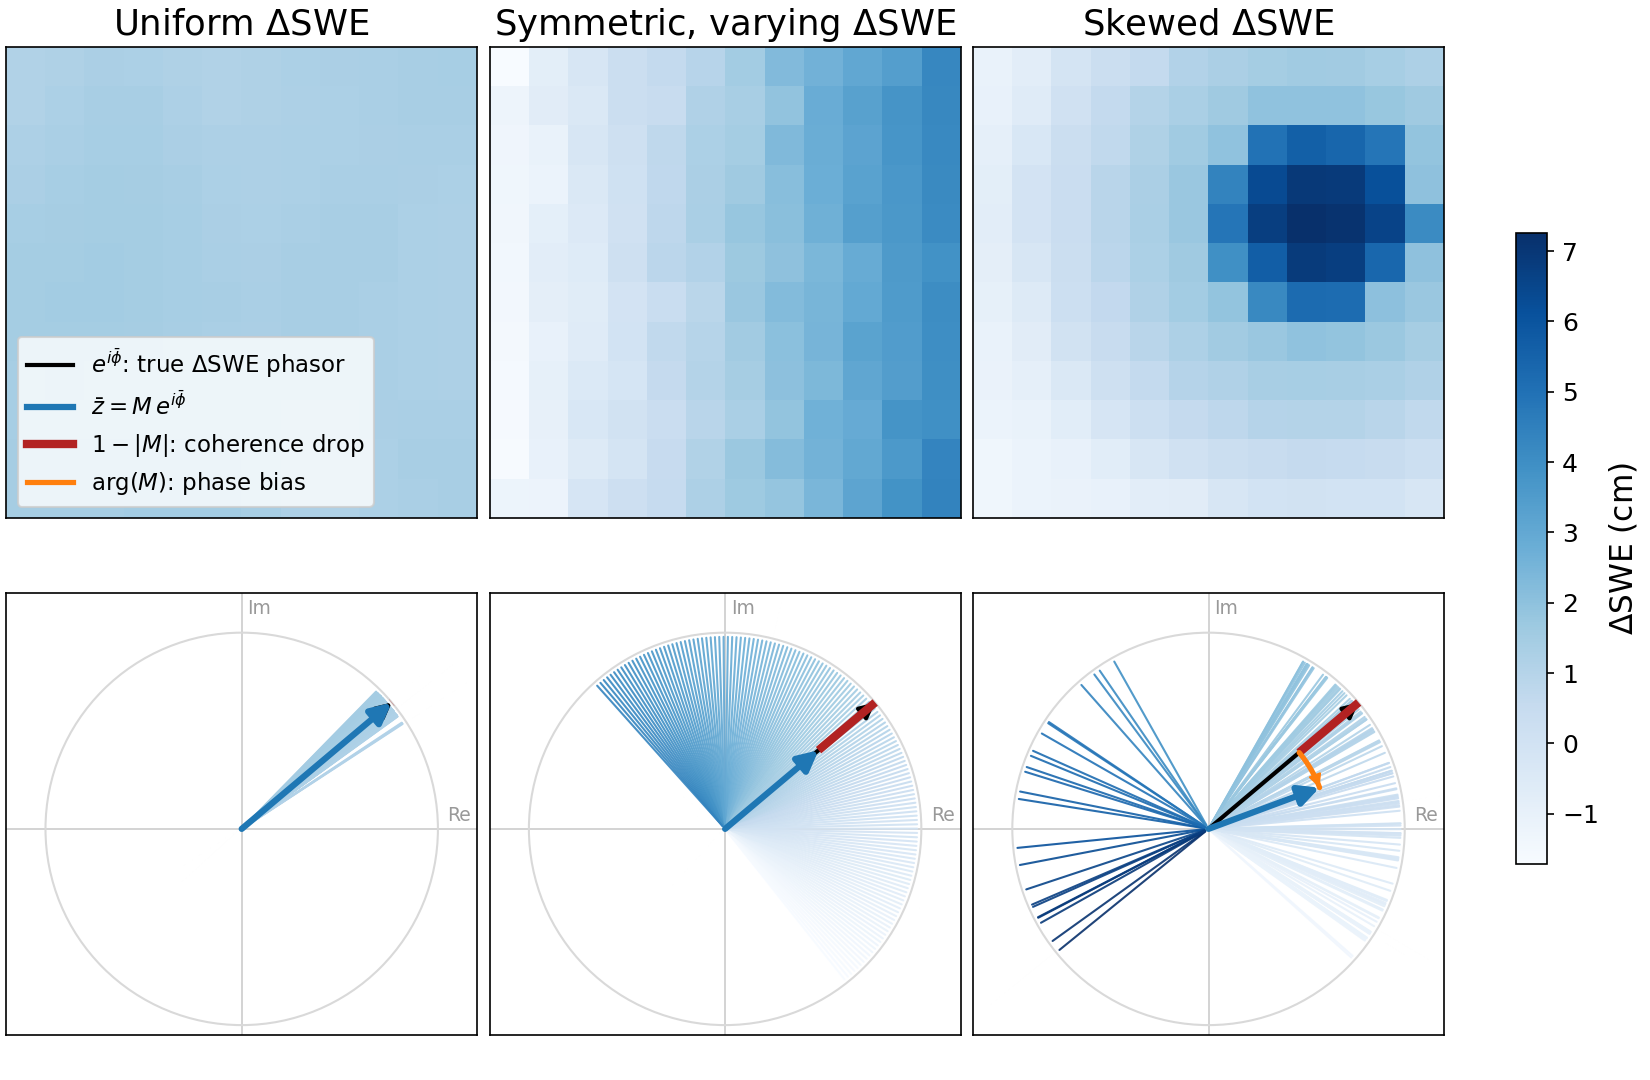
\includegraphics[width=1.0\linewidth]{figures/teach_phasor_contrast.png}
    \caption{Sub-window $\dswe$ variability and its effect on the multi-looked phasor (all other decorrelation removed). \textbf{Top:} $\dswe$ in one window (cm), constant (\textbf{left}), symmetric (\textbf{middle}), and skewed (\textbf{right}). \textbf{Bottom:} per-cell unit phasors ($\phi=\kappa\dswe$, colored by $\dswe$). \emph{Black:} mean phasor $e^{i\bar\phi}$; \emph{blue:} resultant $\bar z=Me^{i\bar\phi}$; \emph{red:} coherence loss $1-|M|$; \emph{orange arc:} retrieval bias $\arg(M)$.}
    \label{fig:theoretical_example}
\end{figure}

The snow-variability coherence loss ($|M|$)  is independent of other decorrelation terms (temporal, geometric, SNR, scattering), so it multiplies ($\gamma_{\rm other}$) to produce the observed decorrelation ($\gamma\rsub{obs}$):

\begin{equation}
    \gamma_{\rm obs} = \gamma_{\rm other}  |M|
\end{equation}

\noindent $\arg(M)$ is the bias of the observed window-mean phase relative to the phase expected from the window-mean $\dswe$, $\kappa\overline{\dswe}$. This bias applies even for a perfectly recovered window-mean phase:

\begin{equation}
    \dphi_{\rm obs} = \kappa\overline{\dswe} + \arg(M)
\end{equation}

Both terms depend only on the within-window distribution of $\dswe$, so they can be computed from any sufficiently fine $\dswe$ map. In the following sections, we compute them from lidar-differenced snow surveys.

\section{Methods}\label{sec:methods}

\subsection{Study Area and Time Frame}\label{subsec:aoi-timeframe}

We target the Tuolumne River basin in the Sierra Nevada (upper Tuolumne and Lyell drainages, 1500--3970~m elevation, $\sim$95$\times$56~km). We use four Airborne Snow Observatory (ASO) lidar pairs bracketing dominant winter accumulations of water years 2023--2026: 2--16 March 2023 (14~d), 29 January--27 February 2024 (29~d), 8--25 February 2025 (17~d), and 31 January--27 February 2026 (27~d). Pair durations were chosen to approximate the NISAR 12-day repeat baseline (one to two repeat cycles per pair) so that the lidar-derived $\dswe$ is representative of what a single NISAR GUNW would measure.

For NISAR data, we use descending track 069, frame 042 over the same basin. Three repeat passes on 7, 19, and 31 December 2025 form two consecutive 12-day interferometric pairs. No ASO flight pair is coincident with these dates, so we characterize the per-interval snow signal from daily SWE at four Tuolumne-basin CDEC pillows (Dana Meadows, Tuolumne Meadows, Slide Canyon, and Gin Flat). December 7 to 19 spans a slight ablation window (mean $-1$~cm SWE change), while December 19 to 31 captures a large December storm (mean $+18$~cm SWE change).

\subsection{Calculation of ASO-$\dswe$}\label{subsec:aso-phase}

ASO delivers snow depth at 3~m and SWE at 50~m, and all flights for a given basin share a common UTM-11N 3~m raster, so pair differencing requires no resampling. For each pair, we form the 3~m $\Delta$depth field $d_B - d_A$ and convert to $\Delta$SWE via a basin-constant new snow density $\rho_{\rm event}$ calculated as the pair's mean of per-pixel $\Delta$SWE/$\Delta$depth ratios from the 50~m ASO products, taken over cells where $|\Delta\text{depth}|\geq10$~cm and the implied density lies in $[50, 600]$~kg,m$^{-3}$: 304, 312, 373, 330~kg,m$^{-3}$ for WY2023--2026. Cells where neither flight has $\geq$10~cm of snow at 50~m resolution are masked from the $\Delta$SWE maps. These densities reflect that the measured snow changes are accumulation with significant settling over the 14--29 day temporal baselines. This approach allows us to take advantage of ASO data with the highest spatial resolution while still centering our analysis around SWE, not snow depth. We block-average the 3~m $\dswe$ field in non-overlapping 3$\times$3 blocks to a 9~m pixel size to suppress any lidar noise (Appendix~\ref{appendix:noise}).

\subsection{Sub-window $\dswe$ Spectral Structure}\label{subsec:psd}

To identify the spatial scales over which the $\dswe$ field varies, we compute its radial power spectral density following the snow-depth fractal analyzes of \citet{trujillo2007topographic-0ec}. This spatial frequency analysis calculates how $\dswe$ variance is distributed across spatial scales and tests whether we would expect significant sub-window variability. We test over spatial frequencies from 9 to 380~m. We run the analysis on the native 3~m field rather than the 9~m working grid because the break can fall below the 18~m Nyquist wavelength of the 9~m grid and be unresolvable there.  Working on the native 3~m field includes the per-pixel ASO depth noise in the spectrum, which we address in Section~\ref{appendix:noise}. A single basin-wide spectrum incorporates many terrain types which blurs any scale breaks, so we work within within smaller windows that span a narrower range of elevation, terrain roughness, and vegetation, the topographic and canopy properties shown to control snow-depth scaling. We tile the common snow mask (cells with valid $\dswe$ in all four pairs) into non-overlapping 1.15~km windows (384 cells on a side) on the native 3~m grid and keep windows that are at least 95\% snow-covered. This window size holds three full cycles of the longest fitted wavelength (380~m) while staying small enough to remain locally homogeneous. Within the retained windows, any invalid cells (at most 5\% of a window) are filled with the window mean. For each window and each ASO pair, we remove the window mean, apply a Hann taper, and form the two-dimensional periodogram as a function of spatial wavenumber $k$ (cycles~m$^{-1}$) \citep{harris1978windows}. We apply no higher-order detrend beyond this mean removal because subtracting a planar trend suppresses the longest-wavelength power and biases the large-scale slope \citep{deems2006}.

The four ASO pairs span an order of magnitude in mean $\dswe$, so a direct average of their spectra would be dominated by the largest-accumulation pair. We instead amplitude-normalize each window's spectrum, subtracting its mean log power over the fitted power spectral density wavelength range of 9 to 380~m before averaging the four pairs' log spectra, which isolates the shared spectral shape. We fit each window's mean spectrum with a continuous two-segment power law, $P(k)\propto k^{-\beta}$, using linear least squares in log--log space weighted by the number of frequencies sampled in each radial bin. The innermost bins average only a few frequencies each, so in an unweighted fit, these few noisy values would control the large-scale slope. The scale break is optimized over spatial wavelengths $\ell=1/k$ from 12 to 250~m, and the break wavelength $\ell_b$ is where the small-scale and large-scale regimes meet. We record a small-scale slope, a large-scale slope, and $\ell_b$ for each window. We also fit each pair separately to test whether the break is consistent across the four winters.

\subsection{Calculation of $M$}\label{subsec:calc-M}

For each ASO-derived $\dswe$ field, we compute the complex sub-window factor $M$ defined in Section~\ref{sec:theoretical-framework}. All processing steps in this section work on a common grid in UTM zone 11N (EPSG:32611) with the origin (upper-left corner) at x = 212352 m, y = 4234641 m.

The $\dswe$ map for each ASO pair is converted to $\dphi$ using NISAR's central frequency (1.26 GHz) and a 40$^{\circ}$ local incidence angle, giving a $\kappa$ of 52.7 radians per meter of $\dswe$, then wrapped onto ($-\pi$, $\pi$). The 40$^{\circ}$ local incidence angle is chosen to represent a moderate incidence angle across NISAR's typical range, but we note that $\kappa$ is sensitive to this choice \citep{Leinss2015}.

We then form the complex variability factor $M$ from non-overlapping $9\times9$-pixel (81~m) windows of $\dphi$, approximately matching the 80~m GUNW posting:
  
\begin{equation}\label{eq:calc_m}
    M = \frac{1}{N}\sum_{n=1}^{N} e^{i(\dphi_n - \overline{\dphi})},
\end{equation}

where $\dphi_n = \kappa\dswe_n$, $\overline{\dphi} = \kappa,\overline{\dswe}$, $\overline{\dswe}$ is the mean $\dswe$ in the window, and $N$ is the number of snow-covered pixels in the window. This is the theoretical Equation~(\ref{eq:def_m}) reformulated to incorporate the mean ASO $\dswe$ within the window. We retain $|M|$ and $\arg(M)$ for windows with $N \geq 41$ (at least half of the pixels are snow-covered).

We repeat the $M$ calculation at two additional wavelengths: C-band (Sentinel-1, $\lambda = 5.6$~cm) and P-band ($\lambda = 81$~cm). The pipeline is unchanged: the same 9~m pre-averaged $\dswe$ field and 81~m windows are used, and only $\kappa(\lambda,\theta)$ (Equation~\ref{eq:dswe2dphi}) is reevaluated for each wavelength, giving $\kappa = 224.1$ and $15.5$~rad,m$^{-1}$ for C- and P-band, respectively. This produces $|M|$ and $\arg(M)$ maps at 81~m for each band and each ASO pair.

Figure~\ref{fig:phase_wraps_bands} shows the wrapped phase response across 0 to 50~cm of $\dswe$ at C-, L-, and P-band, with the basin-mean $\pm$ standard deviation of 50~m ASO $\dswe$ for each pair marked to indicate where each pair sits relative to the wrap interval at each band.

  \begin{figure}
      \centering
      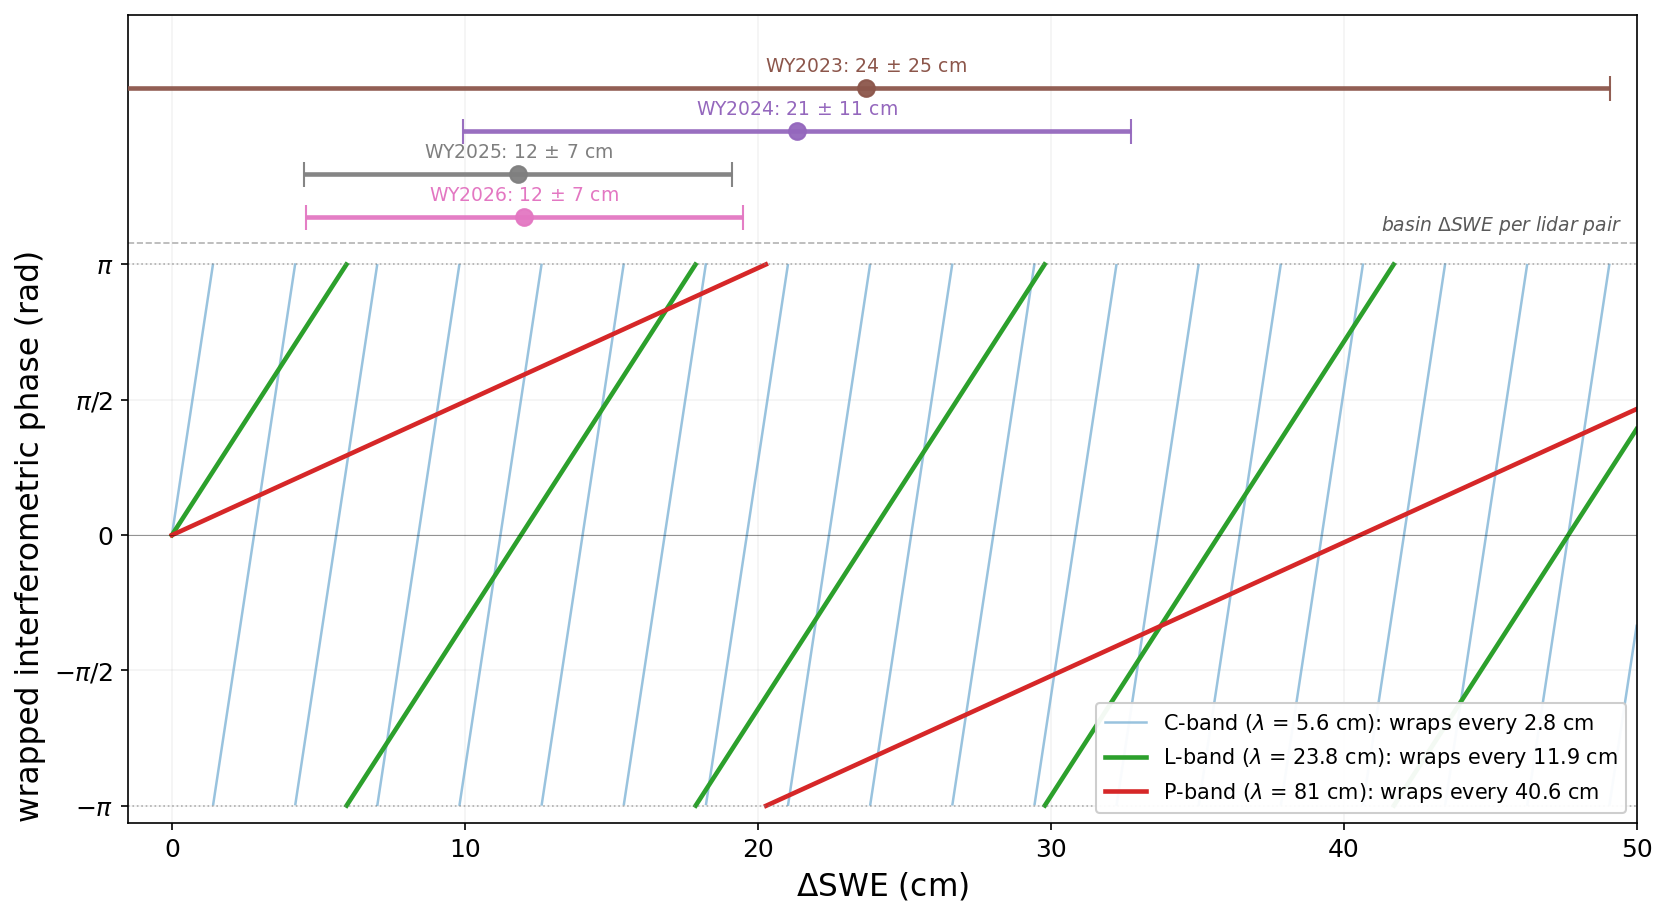
\includegraphics[width=1.0\linewidth]{figures/fig_phase_wraps_bands.png}
      \caption{Wrapped interferometric phase response to $\Delta$SWE accumulation 0 to 50~cm at C-band ($\lambda = 5.6$~cm, blue), L-band ($\lambda = 23.8$~cm, green), and P-band ($\lambda = 81$~cm, red), all at $\theta = 40^\circ$ local incidence angle. Each band's phase increases linearly with $\Delta$SWE at the phase rate $\kappa(\lambda, \theta)$ (Equation~\ref{eq:dswe2dphi}) until it wraps back through $-\pi$. Error bars at the top mark the basin-mean $\Delta$SWE $\pm$ standard deviation for each of the four Tuolumne ASO pairs (50~m basin statistics).}
      \label{fig:phase_wraps_bands}
  \end{figure}

\subsection{Sensitivity of $M$ to Window Size}\label{subsec:sensitivity-of-m-to-window-size}

To trace how the sub-window decorrelation changes with footprint size, we recompute the window factor $M$ over a range of multi-look window sizes on the 3~m $\dswe$ field. The window construction follows Section~\ref{subsec:calc-M}. Here the window size is swept from 9 to 81~m, and unlike Section~\ref{subsec:calc-M} the field is not pre-averaged to 9~m so the smaller windows are resolved. The four ASO pairs are restricted to a common snow mask, the per-pixel intersection of their four valid-$\dswe$ footprints on the shared 3~m grid, so each is evaluated over an identical pixel set. We pool the windows across the four pairs at each size and report the median and interquartile range of $|M|$ and of the L-band SWE-equivalent bias $\arg(M)/\kappa$. The bias is reported only for windows with $|M|>0.3$, since below it $\arg(M)$ is near-uniform over $(-\pi,\pi]$ and carries no recoverable signal. Working on the native 3~m field folds the per-pixel ASO depth noise into $|M|$, which we address in Section~\ref{appendix:noise}.

\subsection{NISAR Multi-resolution Coherence Calculations}\label{subsec:nisar-coherence-calc}

The coherence loss due to sub-window $\dswe$ variability can, in principle, be estimated directly from an interferogram by comparing coherence calculated over different window sizes. The underlying ensemble coherence of a pixel does not depend on the estimation window, but the estimated coherence is affected by two competing, window-size-dependent effects: a positive bias from estimating coherence magnitude with a finite number of looks, which grows as the window shrinks \citep{Bamler1998}, and a negative effect from the sub-window variability of the $\dswe$ signal, assumed in this study to be the dominant source of non-stationarity, which grows as the window expands to span more $\dswe$ variability. Because the finite-look bias is analytically known, we can correct each window size and use the remaining coherence difference between window sizes to estimate the potential sub-window $\dswe$ contribution.

We use the coherence magnitude delivered in each GUNW: the 20~m layer from the wrapped-interferogram group and the 80~m layer from the unwrapped-interferogram group. The expected sample coherence $\hat{\gamma}$ for true coherence $\gamma$ and looks $L$ is given by Equation 62 of \citet{Bamler1998}: 

\begin{equation}
\mathbb{E}\!\left\{\hat{\gamma}\mid\gamma,L\right\}
= \frac{\Gamma(L)\Gamma\!\left(\tfrac{3}{2}\right)}{\Gamma\!\left(L+\tfrac{1}{2}\right)}\;
{}_{3}F_{2}\!\left(\tfrac{3}{2},L,L;L+\tfrac{1}{2},1;|\gamma|^{2}\right)
\left(1-|\gamma|^{2}\right)^{L},
\label{eq:bamler}
\end{equation}

\noindent where $\Gamma$ is the gamma function and ${}_{3}F_{2}$ the generalized hypergeometric function. Equation~\ref{eq:bamler} also assumes circular-Gaussian speckle from a distributed target, which is a reasonable approximation over snow and mixed terrain but a limitation of using this equation. NISAR multi-looks the full-resolution interferogram in radar coordinates independently for each layer (5$\times$6 for the wrapped layer, 13$\times$16 for the unwrapped layer) and then geocodes each layer onto its delivered map grid. The geocoding resamples the multi-looked pixels, so neighboring samples on the 20 and 80~m grids are partially correlated and the nominal look counts ($N = 30$ at 20~m, 208 at 80~m) overstate the number of independent samples. We therefore use an effective look count $L=N/f$, with $f$ an oversampling factor calibrated over open water on Don Pedro Reservoir near the study site, where the true coherence is assumed zero at both resolutions. Water pixels are identified as ESA WorldCover permanent-water (class 80) cells with NISAR 80~m coherence below 0.20, the latter cut removing coherent shoreline pixels (13,189 samples). Requiring the bias-corrected 20~m and 80~m water coherences to agree gives $f \approx 1.29$, $L_{20} \approx 23$, and $L_{80} \approx 162$.

We then de-bias each resolution by inverting Equation~\ref{eq:bamler} for the true coherence,

  \begin{equation}
    \tilde{\gamma}_{s} = \mathbb{E}^{-1}\!\left\{\hat{\gamma}_{s}\mid L_{s}\right\},
    \quad s\in\{20,80\},
    \label{eq:debias}
  \end{equation}

\noindent and take the difference of the corrected coherences

  \begin{equation}
    \Delta\gamma = \tilde{\gamma}_{20} - \tilde{\gamma}_{80}
    \label{eq:cohdiff}
  \end{equation}

\noindent as our NISAR estimate of the sub-window-variability coherence loss. With $\gamma_{\rm obs}=|M| \gamma_{\rm other}$ and $\tilde\gamma_{20}\approx\gamma_{\rm other}$, this difference is $\Delta\gamma \approx \gamma_{\rm other}(1-|M|)$, reducing to $1-|M|$ only where the other decorrelation effects are minimal ($\gamma_{\rm other} \approx 1$). Because the 20~m window itself still carries some sub-window loss, $\Delta\gamma$ is a lower bound on the true sub-window coherence loss. 

\section{Results}\label{sec:results}

\subsection{$\dswe$ Power Spectral Densities}\label{subsec:power_spectral_densities}

Resolved per window on the native 3~m grid, the $\dswe$ spatial power spectrum is a two-regime power law with a break at a median wavelength of $\ell_b = 27$~m (IQR 22--31~m across 570 windows; Figure~\ref{fig:psd_break}). The spectrum is steep below the break (median slope $\beta = 2.6$) and shallow above it ($\beta = 1.5$), so the $\dswe$ field is smooth and spatially correlated at scales finer than about 30~m and rougher at larger scales. Fitting each ASO pair separately gives $\ell_b$ between 22 and 27~m, and 88\% of the window breaks fall within the 15--40~m range reported for cumulative snow depth \citep{deems2006}.

\begin{figure}
\centering
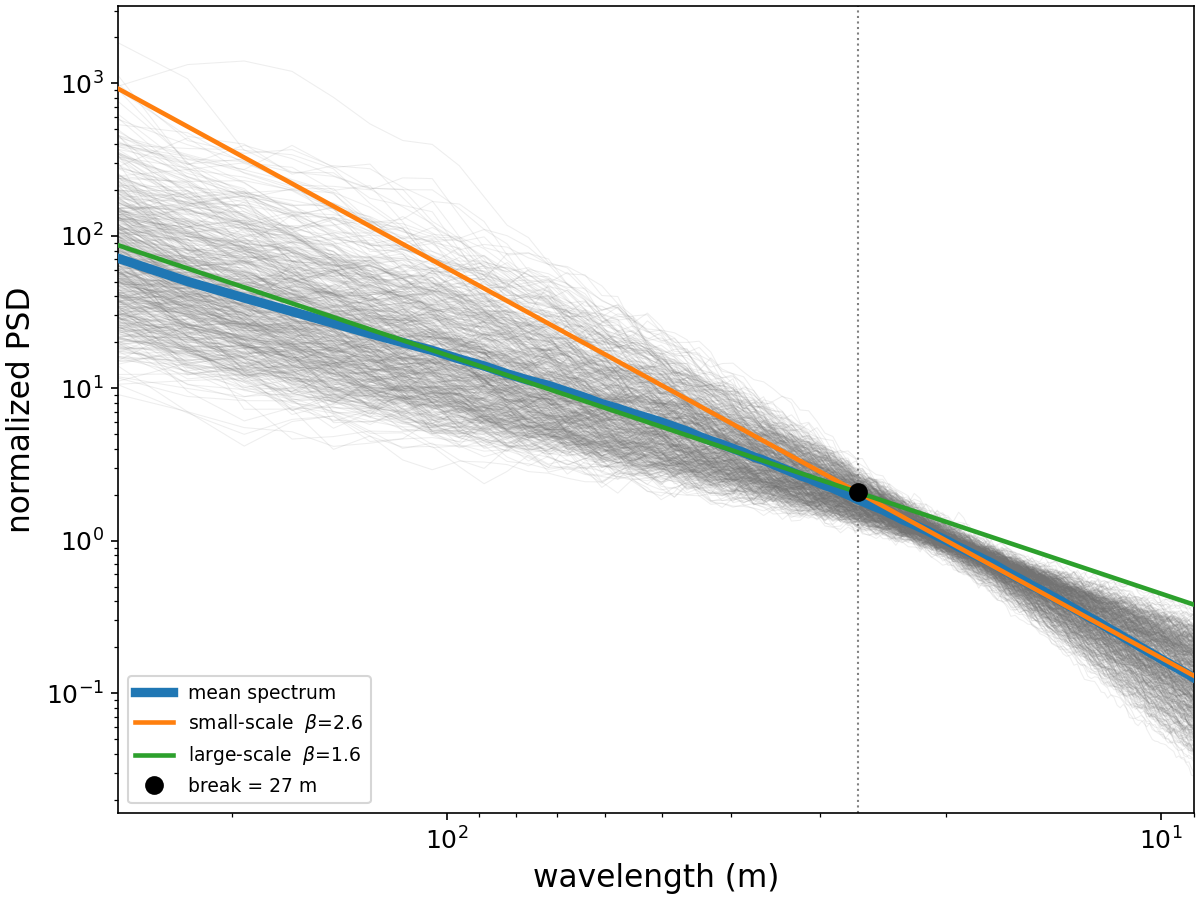
\includegraphics[width=0.7\linewidth]{figures/dswe_psd_break.png}
  \caption{Radial power spectral density of the native 3~m $\Delta$SWE field, for each 1.15~km window, amplitude-normalized and averaged over the four lidar pairs so only the spectral shape is compared. Grey lines are the individual windows, blue is their mean, and the orange and green lines are the fitted small-scale and large-scale segments, $P(k)\propto k^{-\beta}$ with $\beta\approx2.6$ and $1.5$. The segments meet at the break (black point) near 27~m.}
  \label{fig:psd_break}
\end{figure}

\subsection{Lidar Derived Sub-window $\dswe$ Variability Effects}\label{subsec:lidar-variability}

All lidar $\dswe$ statistics in this section are computed over the non-overlapping 81~m windows defined in Section~\ref{subsec:calc-M}. Pooled over the four pairs (1.34 million windows), the window-mean $\dswe$ has a median of 12.6~cm (IQR 4.7--20.4~cm), a within-window median standard deviation of 3.4~cm (IQR 2.1--6.3~cm) and a slight positive within-window skewness (median $+0.07$, mean $+0.14$). The within-window standard deviation captures the sub-window $\dswe$ variability that drives $|M|$, and the within-window skew drives $\arg(M)$.

The four pairs show a consistent, terrain-organized spatial pattern. The coherence loss $1-|M|$ and the bias magnitude $|\arg(M)|$ are both largest in the deep, spatially complex alpine terrain and smallest in the smoother, lower-elevation terrain (Figure~\ref{fig:aso_all_pairs}), and both patterns repeat across pairs, with each pair matching the four-pair mean with $r^2=0.75$--$0.82$ for $|M|$ and $0.59$--$0.63$ for $|\arg(M)|$. The sign of the bias is year-specific (signed $\arg(M)$ pairwise $r^2<0.01$). Its spatial intensity tracks the terrain while its direction varies between events.

Although the basin-median $\dswe$ ranges over an order of magnitude across the four pairs (0.7--23~cm), the coherence drop and bias stay within narrow bands. Median $|M|$ runs from 0.25 (WY2024) to 0.47 (WY2023; pooled IQR 0.15--0.58), and the median retrieval bias is near zero ($\leq2^\circ$) with heavy tails (pooled IQR $\pm16^\circ$, widening to $-17^\circ$/$+30^\circ$ in the largest event, WY2024). The three large mid-winter storms (WY2024--2026) drive median $|M|$ to 0.25--0.31, falling to $\sim$0.12--0.16 in the steep high-elevation terrain, whereas the one melt-dominated pair (WY2023) has the smoothest $\dswe$ field ($\sigma_{\dswe}$ median 2.8~cm), stays closest to stationarity, and shows the highest $|M|$ (0.47) and the least bias (median $\approx0^\circ$). Within WY2023, splitting the windows by the sign of the window-mean $\dswe$ gives the melt windows a median $|M|$ of 0.55 against 0.32 for the accumulation windows, a gap that persists at matched $|\dswe|$ magnitude.

\begin{figure}
  \centering
  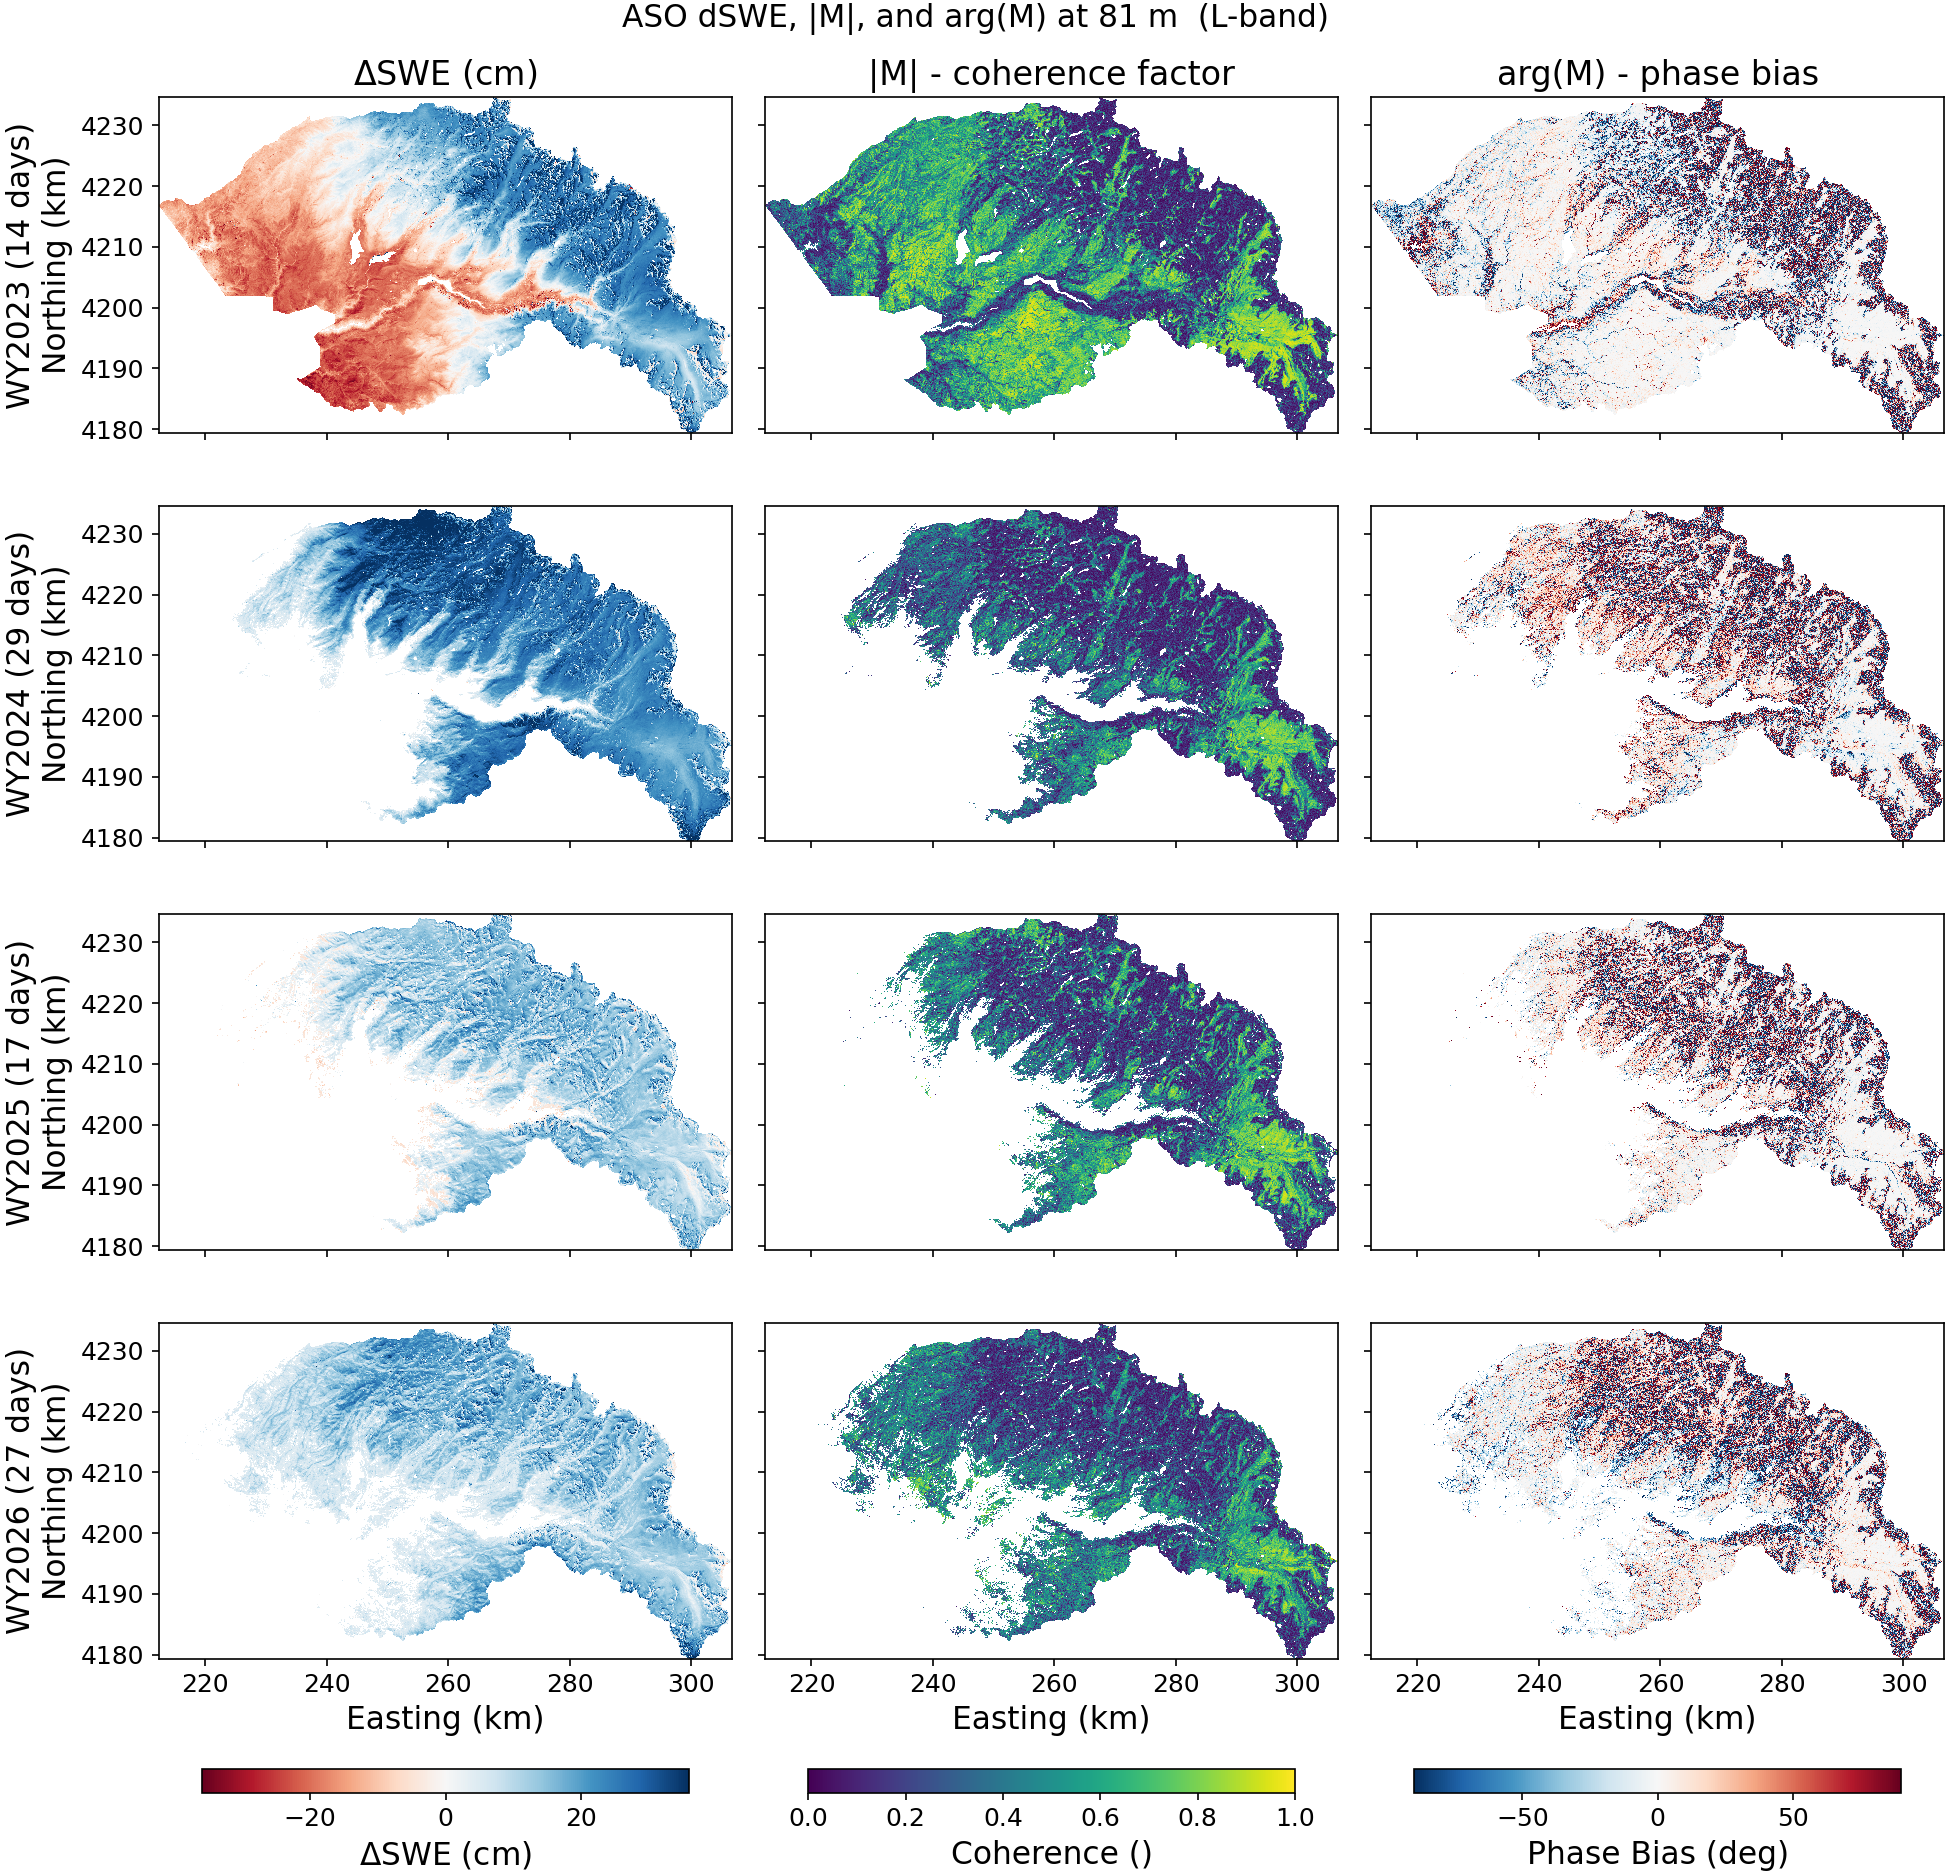
\includegraphics[width=1.0\linewidth]{figures/all_pairs_dswe_M_L.png}
  \caption{Lidar-derived $\Delta$SWE, sub-window coherence factor $|M|$, and retrieval bias $\arg(M)$ at 81~m for the four Tuolumne lidar pairs (rows, labeled by water year and temporal baseline), evaluated at L-band, 40$^\circ$ local incidence angle. Columns: the 81~m block-averaged $\Delta$SWE field (\textbf{left}), $|M|$ (\textbf{center}), and $\arg(M)$ (\textbf{right}).}
  \label{fig:aso_all_pairs}
\end{figure}

\subsection{Coherence Loss and Bias Across Window Sizes}\label{subsec:window-size-results}

The L-band coherence factor falls steeply as the multi-look window grows and then plateaus (Figure~\ref{fig:window_size}, top). The pooled median $|M|$ drops from 0.54 at a 9~m window to 0.33 at 20~m and 0.18 at 81~m, with most of the loss incurred by about 25~m. The interquartile range is wide at every size and stretches further downward as the window grows, spanning 0.07 to 0.38 at 81~m, reflecting the strong terrain control on the sub-window $\dswe$ structure. The two NISAR GUNW postings bracket a large part of the curve. The 20~m wrapped-interferogram footprint retains a median $|M|$ of 0.33 compared to 0.18 at the 80~m footprint, almost double the coherence factor for the same scene.

The L-band retrieval bias stays small across the whole range (Figure~\ref{fig:window_size}, bottom). In usable windows, the median SWE-equivalent bias never exceeds 0.3~mm, and the interquartile range stays within about $\pm2$~mm. The band is slightly asymmetric, with a longer positive tail (the signature of the within-window $\dswe$ skew) but the magnitude is negligible compared to the coherence loss. The bias does not grow significantly at any footprint between 9 and 81~m.

\begin{figure}
  \centering
  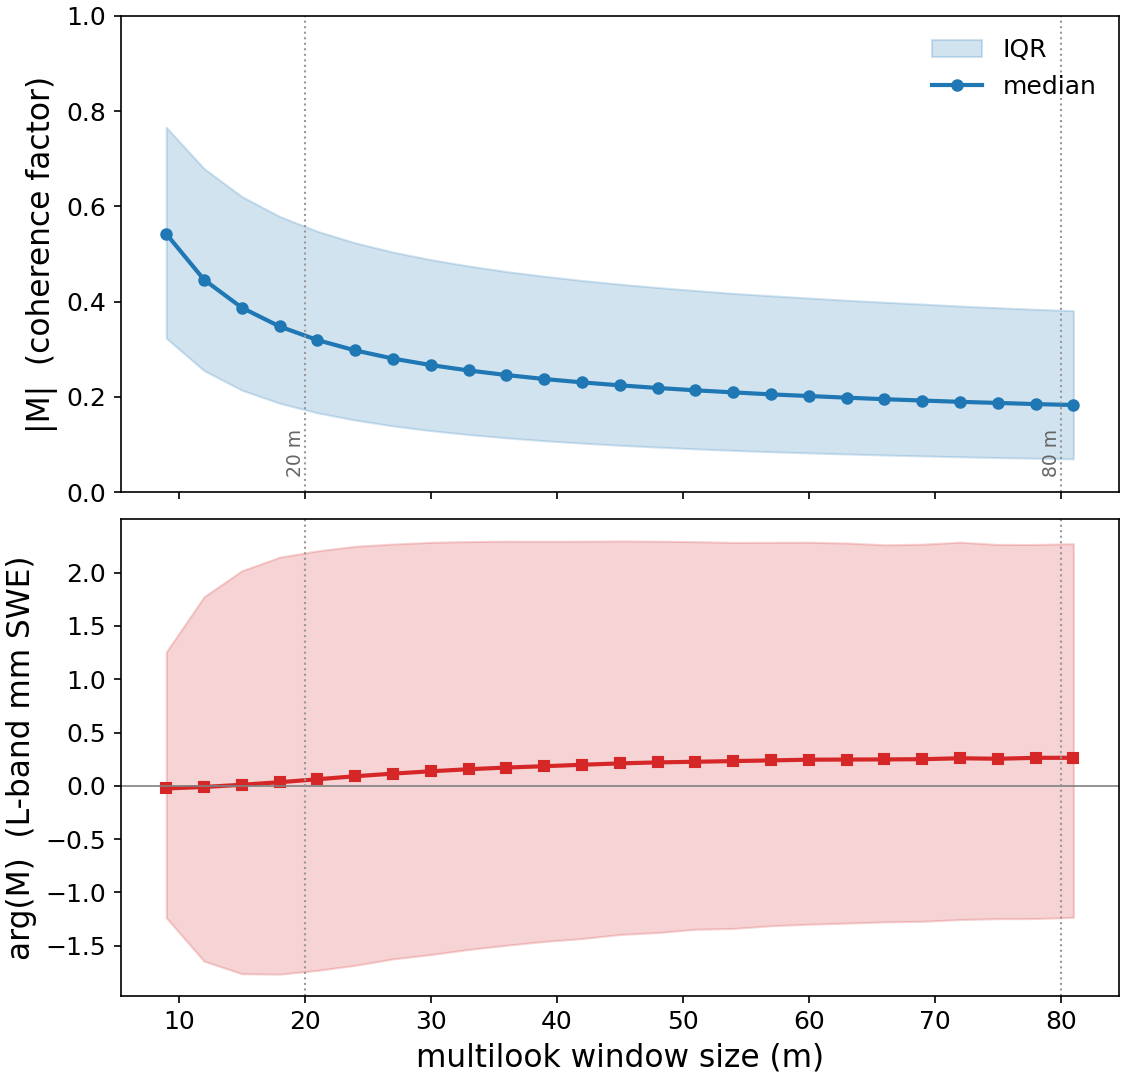
\includegraphics[width=0.8\linewidth]{figures/window_M_arg_vs_size_L.png}
  \caption{Sub-window coherence factor $|M|$ (\textbf{top}) and retrieval bias $\arg(M)$ (\textbf{bottom}) versus multi-look window size, L-band, pooled over the four lidar pairs (median and shaded interquartile range). Computed on the native 3~m $\dswe$ field.The bottom panel is restricted to usable windows ($|M|>0.3$) and converted to an L-band SWE-equivalent through $\arg(M)/\kappa$. Dotted lines mark the 20 and 80~m NISAR GUNW postings.}
  \label{fig:window_size}
\end{figure}


\subsection{NISAR Multi-resolution Coherence}\label{subsec:nisar-coherence}

The corrected $\gamma_{20}-\gamma_{80}$ is near zero for the near zero-SWE-change December 7--19 pair (median $-0.005$, 43\% of windows positive) and positive for the December 19--31 storm pair (median $+0.022$, 66\% positive) over the snow-covered footprint (Figure~\ref{fig:coherence_rows}). Most of the raw $20$--$80$~m gap is finite-look estimation bias. For the December 19--31 pair, the raw gap $+0.072$ (median) is reduced to $+0.022$ by the bias correction, while for the snow-free pair, the corrected gap is close to zero. However, the largest corrected residuals cluster at higher elevations, where more $\dswe$ variability is both expected from the lidar and the observed  NISAR residual is correspondingly larger. For the storm pair, the corrected gap stays small in the median ($\leq0.03$ across elevations), but its upper tail grows with elevation, with the strongest windows (90th percentile) rising to $\sim$0.12 in the highest, most exposed terrain, where the 80~m coherence is also lowest (median 0.16).

\begin{figure}
  \centering
  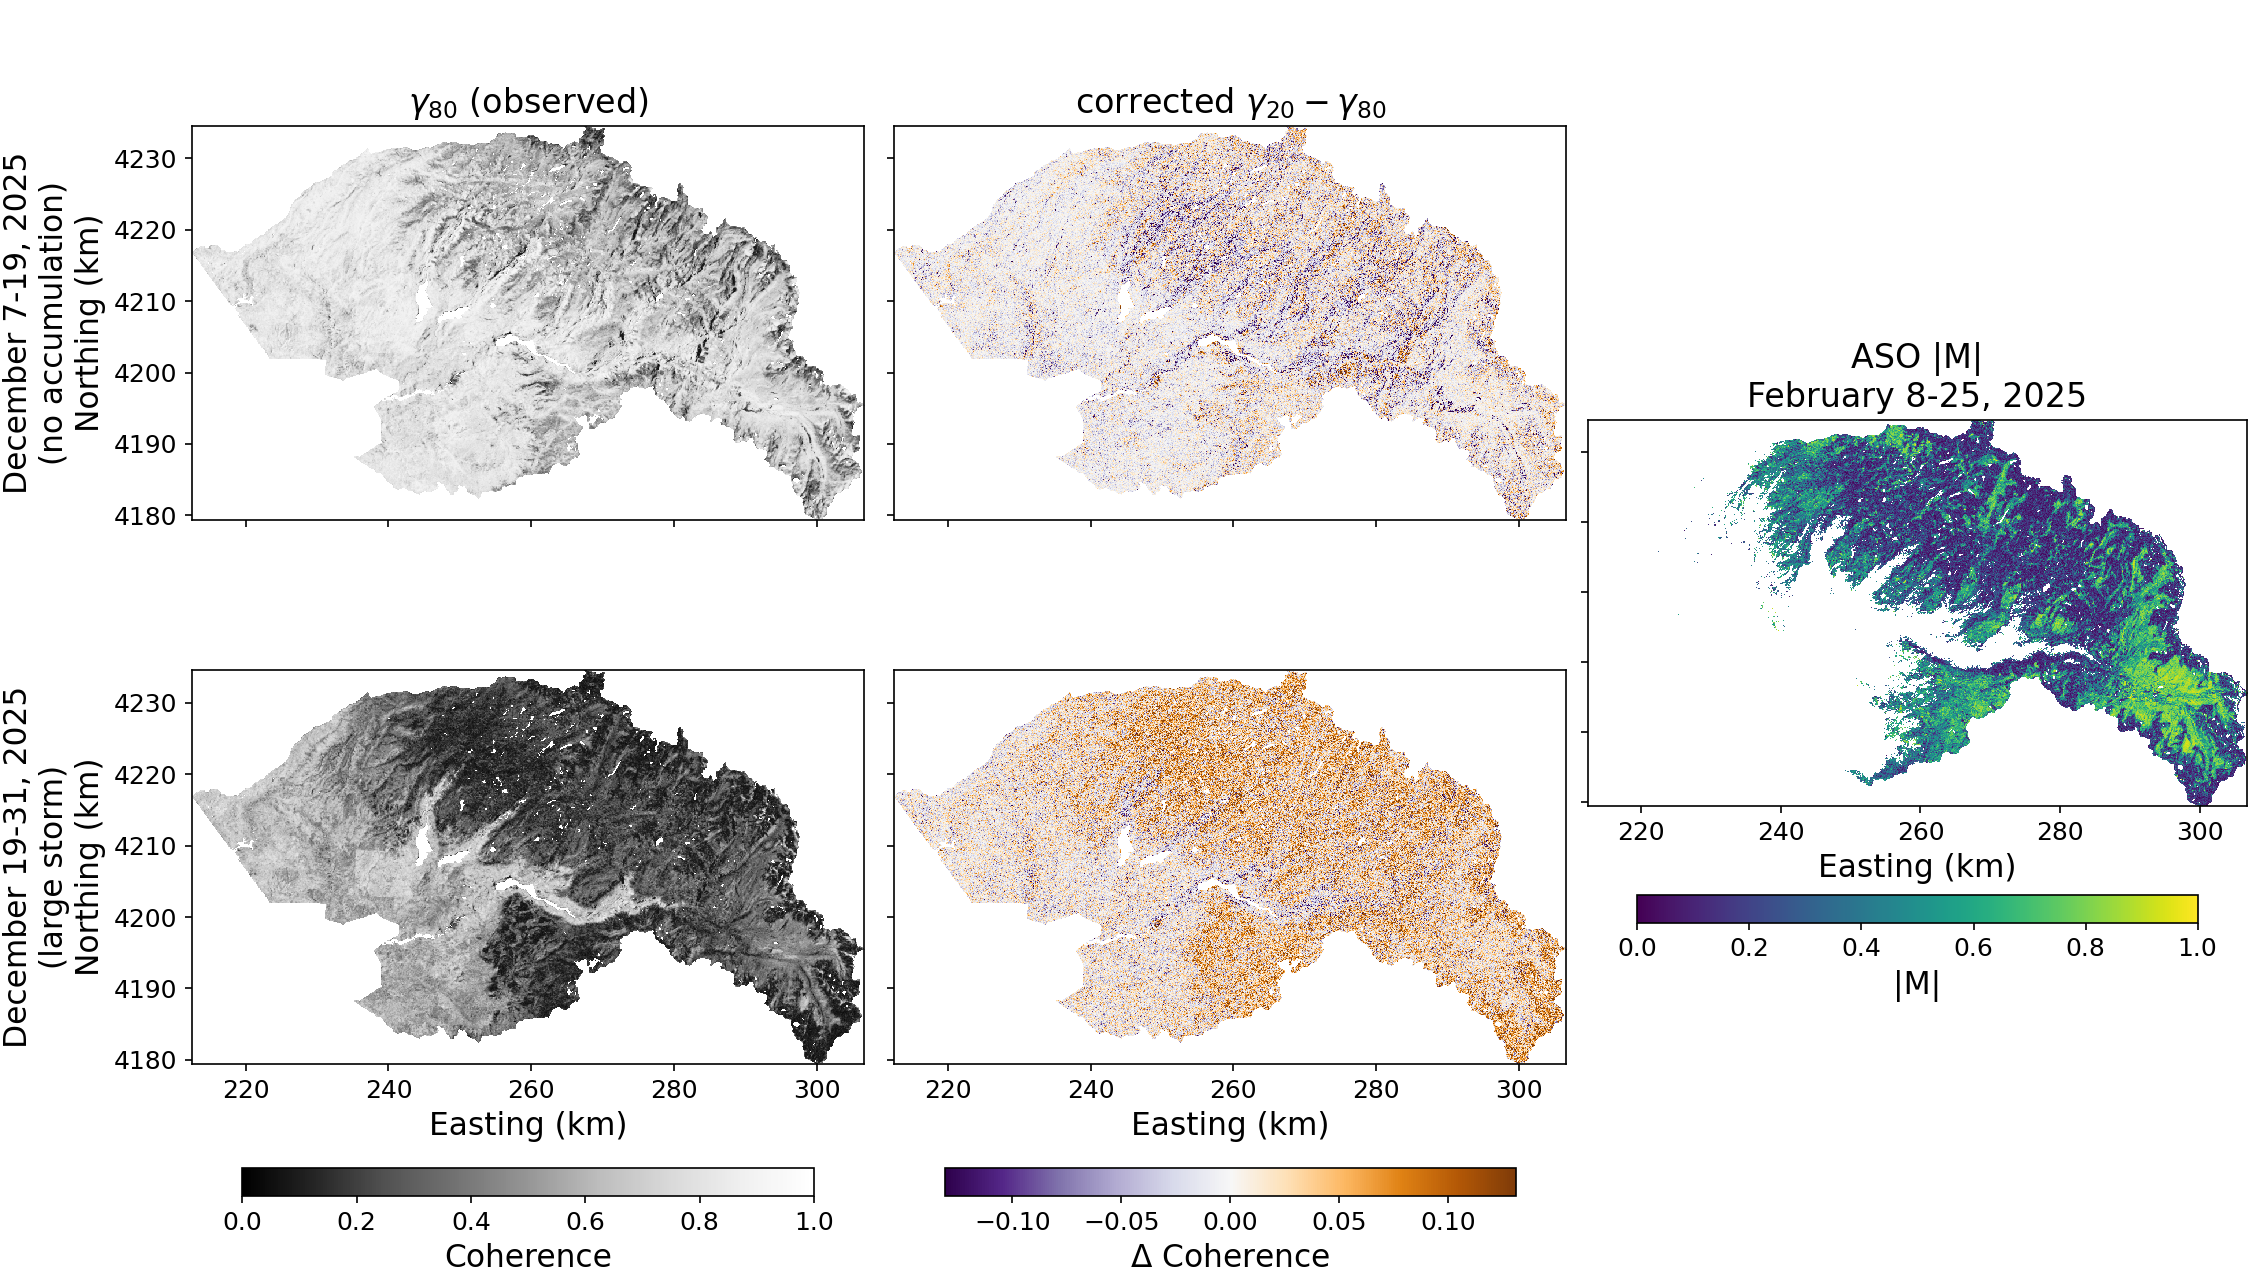
\includegraphics[width=1.0\linewidth]{figures/coherence_rows_P12_P23.png}
  \caption{NISAR multi-resolution coherence for the low-snow P12 (7--19 December 2025) and large-storm P23 (19--31 December 2025) pairs: observed 80~m coherence $\gamma_{80}$ (\textbf{left}), the finite-look-corrected difference $\gamma_{20}-\gamma_{80}$ (\textbf{center}), and the lidar-predicted sub-window coherence factor $|M|$ (\textbf{right}, WY2025), all on the common 81~m grid.}
  \label{fig:coherence_rows}
\end{figure}

\subsection{Wavelength Effect on $M$}\label{subsec:wavelength-M}

The same sub-window $\dswe$ field produces very different effects across bands, because shorter wavelengths turn the same $\dswe$ spread into a larger phase spread and more wrapping (Figure~\ref{fig:M_bands_wy2025}). At C-band ($\kappa = 224.1$~rad,m$^{-1}$) the within-window phase spread is large enough that coherence collapses, with median $|M| = 0.10$ (IQR 0.06--0.14) and 53\% of windows below 0.1. So little coherent signal survives that the retrieval bias is undefined, with $\arg(M)$ distributed nearly uniformly over $\pm90^\circ$, IQR $-86^\circ$ to $+88^\circ$. At P-band ($\kappa = 15.5$~rad,m$^{-1}$) coherence is largely preserved (median $|M| = 0.87$, IQR 0.65--0.94; $<$1\% of windows below 0.1) and the bias is small and well-defined ($\arg(M)$ IQR $-1.6^\circ$ to $+0.3^\circ$). L-band is intermediate, with median $|M| = 0.31$ (IQR 0.15--0.55), 14\% of windows below 0.1, with a small but resolvable bias ($\arg(M)$ IQR $-15^\circ$ to $+19^\circ$). The same ordering holds when data is pooled over all four lidar pairs (median $|M|$ = 0.10 / 0.33 / 0.88 for C/L/P), so that it reflects the wavelength scaling rather than any one event.

\begin{figure}
  \centering
  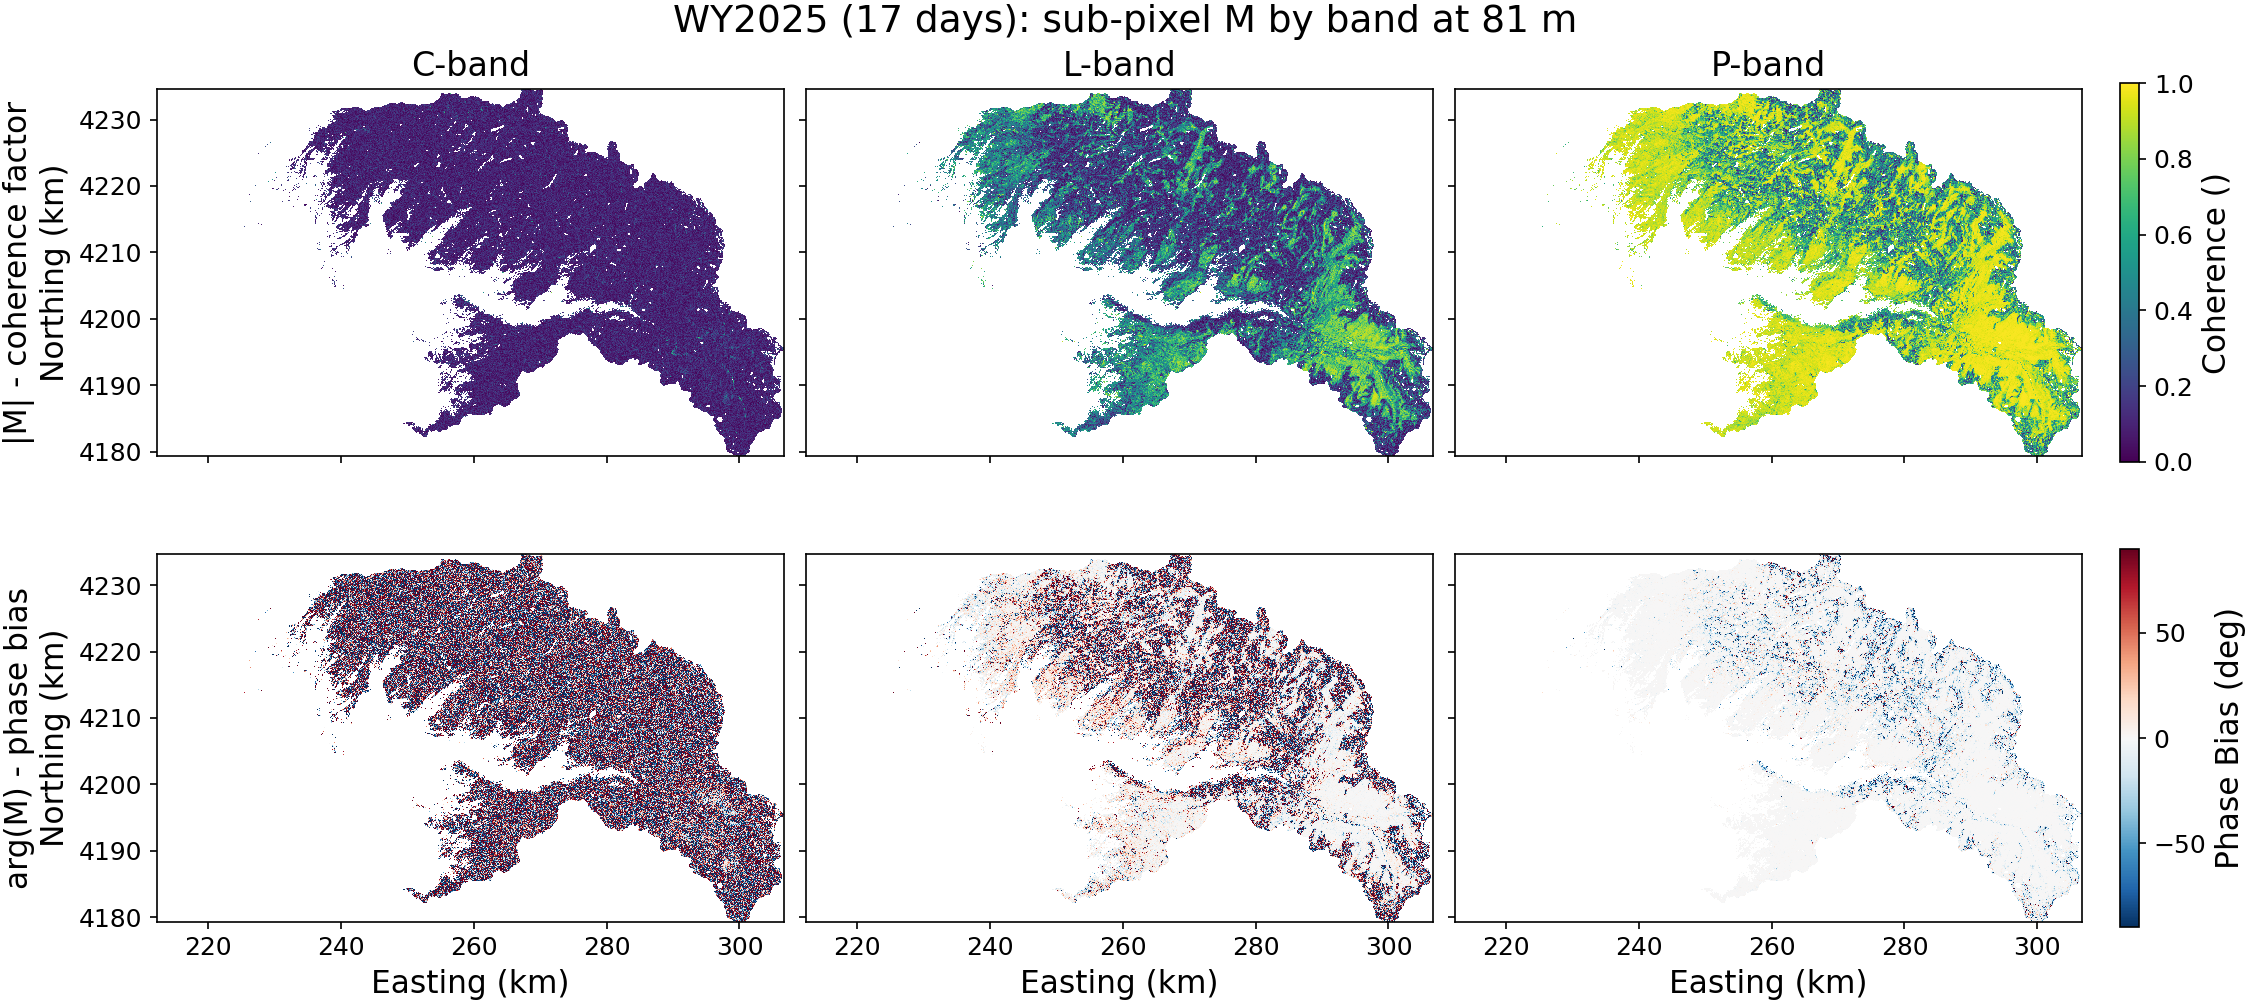
\includegraphics[width=1.0\linewidth]{figures/bands_M_WY2025.png}
  \caption{Sub-window coherence factor $|M|$ (\textbf{top}) and retrieval bias $\arg(M)$ (\textbf{bottom}) at 81~m for the WY2025 lidar pair (8--25 February 2025) at C-, L-, and P-band.}
  \label{fig:M_bands_wy2025}
\end{figure}


\section{Discussion}\label{sec:discussion}

Using repeat lidar surveys and NISAR interferometry, we have shown that within-window $\dswe$ variability reduces coherence and $\dswe$ skew biases the retrieved $\dswe$ from the true mean $\dswe$, both of which degrade InSAR SWE retrievals. Here we consider what these results mean in practice: the length scales at which the $\dswe$ field is organized, the resulting effects at NISAR's standard postings, and how the effect scales from C- to P-band.

\subsection{$\dswe$ Structure and the Processing Window Size}\label{subsec:break-discussion}\label{subsec:window-size-discussion}

The $\dswe$ spectral break at $\ell_b \approx 27$~m falls within the 15--40~m variogram range scale breaks reported for cumulative snow depth and matches the wind- and vegetation-controlled short-scale regime of \citet{trujillo2007topographic-0ec}. The change in SWE between two flights is therefore organized at the same length scales as the snowpack itself, so differencing two snow surfaces preserves the fine-scale structure. This holds in all four winters, so the variability driving within-window phase spread is a persistent feature of accumulation, not an artifact of a single season.

This break sets the window sizes over which the sub-window coherence loss develops. Within-window $\dswe$ variance grows rapidly as the window expands toward $\ell_b$ and more slowly beyond it, so most of the coherence loss is already incurred by the time the footprint reaches a few tens of meters. The 80~m GUNW posting sits well past the break, where the loss has saturated near its maximum. The window-size sweep shows the same behavior in $|M|$ directly. The empirical curve is steepest below about 25~m and flattens beyond, with the slope change near the spectral break. Moving from the 80~m GUNW posting to a 20~m footprint nearly doubles the median $|M|$, from 0.18 to 0.33. The coherence recovered per step keeps growing as the window shrinks toward $\ell_b$, so even modest reductions below the GUNW default return usable coherence over the spatially variable snow that decorrelates the 80~m product.

The bias result simplifies the choice. Across the full 9 to 81~m range, the SWE-equivalent bias in usable windows stays at the millimeter level, far below the coherence loss and below the retrieval uncertainty from other sources. The footprint is therefore a coherence tradeoff and not a bias tradeoff. A larger window loses coherence without incurring a meaningful retrieval bias in the pixels that survive a coherence threshold, and a smaller window recovers coherence without introducing bias. The footprint should be chosen to keep $|M|$ usable over the target snowpack, and the residual skew-driven retrieval bias can be neglected in any window that passes a coherence mask.

Shrinking the window has a limit. Smaller windows average fewer pixels, so the random phase noise that multi-looking suppresses, whose variance falls as $1/N$ with the number of looks \citep{Bamler1998}, rises as the footprint shrinks. The best footprint balances the recovered sub-window coherence against this estimation noise and is set by the local $\dswe$ correlation length, the $\ell_b \approx 27$~m break, rather than a fixed look count. For these Tuolumne events that balance sits well below the 80~m GUNW posting, and large accumulation events such as the December 2025 storm need the finest practical footprint to keep the sub-window term in check. The most wind-exposed terrain, where short-scale variance is largest, will remain the hardest to recover at any footprint.

\subsection{Snow-based Multi-look Coherence Bias}\label{subsec:coherence-bias}

Coherence measured over seasonal snow has historically been interpreted through a decorrelation budget of temporal, geometric, SNR, and volume terms, with residual loss most often assigned to temporal decorrelation of the snow volume \citep{Ruiz2021, Oveisgharan2024}. The presented sub-window $\dswe$ effect is itself a change-driven decorrelation, since it arises from the snow that accumulates between passes, but it differs from the usual temporal term: rather than the stochastic motion of sub-resolution scatterers within a cell, it is the deterministic variation of the resolved $\dswe$ field across cells within the multi-look window. Our lidar-derived $|M|$ maps show that a substantial share of the L-band coherence drop over an accumulation interval is this deterministic sub-window component rather than stochastic temporal decorrelation. Because it is set by the resolved snow structure, it can be predicted from lidar and reduced by processing at a finer footprint, neither of which is true of the stochastic temporal term to which it is usually attributed.  Across the four Tuolumne lidar pairs, the sub-window factor lowers the basin-median $|M|$ to 0.25--0.47 (Figure~\ref{fig:aso_all_pairs}) at an 81~m window, a coherence loss of 0.5 to 0.75 carried by within-window $\dswe$ structure before any temporal or thermal term is applied. 

Turning to the NISAR data, both the raw coherence and the multi-resolution residual show the temporal and spatial patterns that these lidar $\dswe$ results predict. The raw 80~m coherence is lower for the December 19--31 storm pair than for the near-snow-free December 7--19 pair, and within the storm pair it is lowest over the steep alpine terrain where sub-window $\dswe$ variability is greatest (median $\gamma_{80}\approx0.16$ at the highest elevations versus $\approx0.27$ at the lowest). Raw coherence alone cannot separate the sub-window loss from other decorrelation, but the corrected $\gamma_{20}-\gamma_{80}$ residual repeats both patterns where only the sub-window term should appear. It is near zero for the no-accumulation pair (median $-0.005$), positive for the storm pair (median $+0.022$ over snow), and largest in the highest, most complex terrain. The observed residual is smaller than the lidar-predicted gap ($|M|_{20}-|M|_{80}\approx0.15$, Section~\ref{subsec:window-size-results}) because $\gamma_{\rm other}$ multiplies the difference and much of the storm-pair scene is decorrelated enough that the gap is lost to phase noise. In the most variable high terrain, where the prediction is largest, the corrected residual approaches 0.1 (90th percentile 0.12). Coherence over snow may therefore be misattributed to temporal decorrelation when part of it is a within-window phase-variability signal.

Even at a finer footprint, the retrieval is more tractable where the $\dswe$ field is smooth. The $|M|$ drops to 0.12–-0.16 in the steep, wind-exposed alpine drainages but stays near one over the lower-elevation, gently varying terrain (Figure~\ref{fig:aso_all_pairs}, center column). This terrain control holds across events. The basin-median $\dswe$ spans an order of magnitude across the four pairs, while the median $|M|$ stays within a narrow band, so the decorrelation and bias are set by terrain and snowpack structure rather than by event size. Since some multi-looking will be necessary to improve phase estimates, retrievals will work best when targeted at regions and snowpacks whose $\dswe$ varies gently relative to the multi-look window. The most variable alpine terrain may be unrecoverable at any current spaceborne footprint.

Melt periods may be more favorable than accumulation for the sub-window term considered here. Once the snowpack has ripened and refrozen, melt-driven $\dswe$ varies smoothly with elevation and aspect rather than in wind-built drifts, which keeps the within-window variance and skew low. The WY2023 melt-versus-accumulation split (Section~\ref{subsec:lidar-variability}) shows this directly, with the gap persisting at matched $|\dswe|$ magnitude and driven by a lower within-window spread, so melt removes SWE more uniformly within the window than wind deposits it. This smoother sub-window signal only helps if the wet-snow dielectric and temporal decorrelation terms in $\gamma_{\rm other}$ do not collapse the coherence on their own. L-band ablation retrievals have been initially demonstrated for morning refrozen acquisitions \citep{Tarricone2023}, but they will be sensitive to the estimated liquid water content, as this impacts the radar wave speed and, therefore, the phase.

This mechanism also explains why wind is the single largest control on snow coherence in \citet{Ruiz2022}. Wind is the main agent of fine-scale snow redistribution, building dunes, scour, and drifts at length scales well below typical multi-look window sizes \citep{trujillo2007topographic-0ec}. This redistribution raises the within-window $\dswe$ variance and skew, which shortens and rotates $M$, so a windy interval produces the asymmetric, sub-window $\dswe$ distribution that Figure~\ref{fig:theoretical_example} identifies as the source of both coherence loss and retrieval bias. This is the same mechanism \citet{LiSturm2002} identified at C-band, where mapped ERS-1 coherence loss tracked the spatial and temporal patterns of wind-driven redistribution, and that \citet{ming2026} found for C-band over first-year sea ice by decomposing the coherence budget. Our results confirm both findings from lidar rather than from the interferograms themselves. At C-band, the wavelength examined by \citet{LiSturm2002} and \citet{ming2026}, $|M|$ collapses to a median of 0.10, and the lowest $|M|$ in every pair falls in the wind-exposed alpine terrain. The dominance of wind as a predictor in \citet{Ruiz2022} is what we would expect if sub-window $\dswe$ variability, rather than bulk temporal changes affecting temporal coherence, governs the observed coherence.

\subsection{Skew-Drive Retrieval Bias Considerations}\label{subsec:phase-bias}

The sign of the retrieval bias is set by the skew of the within-window $\dswe$ distribution (Figure~\ref{fig:theoretical_example}). Before the phase wraps, a positively skewed distribution produces a negative retrieval bias, which rotates the multi-looked phase below the true window-mean phase and results in a lower retrieved  $\dswe$ than the true mean in those windows. A physically likely source of this positive skew is wind loading: a few wind-loaded pixels carry much more new snow than the rest of the window and sit as positive outliers in an otherwise smooth $\dswe$ field, lengthening the right tail of the distribution.

The lidar-derived $\arg(M)$ maps show the same pattern (Figure~\ref{fig:aso_all_pairs}, right column). The retrieval bias is a real effect, but it is a small one. It is near zero across most of the basin and rises only in the steep, wind-exposed alpine terrain, where the within-window variability is largest and the coherence is lowest. This $\dswe$ bias is therefore largest exactly where the phase is least reliable. In SWE terms, it stays near $\pm5$~mm (converting phase to L-band $\dswe$ bias) across the basin and reaches about 1.5~cm only in the most wind-affected windows of the largest event. Because the bias peaks with the coherence loss, pixels that pass a coherence threshold carry little bias, so it mostly affects pixels that may already be unusable. This coupling only holds at shorter wavelengths. At longer wavelengths, the coherence is preserved while the bias remains, which we turn to below.

\subsection{C-, L-, and P-band Analysis}\label{subsec:band-analysis}

P-band is appealing for SWE retrieval. The smaller $\kappa$ keeps coherence high over the large accumulation events that decorrelate L-band. However, at P-band, the retrieval bias is still present and consistently negative ($\arg(M)$ IQR $-1.6^\circ$ to $+0.3^\circ$), and it is the one band where the bias is not correlated with almost complete coherence drops. The negative sign is the one predicted for a positively skewed $\dswe$ distribution, and it appears here because the longer wavelength keeps the within-window phase spread small enough that the multi-looked phase does not wrap. At C- and L-band, the same bias is present but masked since the larger phase spread wraps and pulls the median $\arg(M)$ back toward zero. A longer-wavelength sensor has a narrower window phase distribution, but where that assumption breaks down in the steep alpine terrain, it carries a systematic negative bias without the matching total coherence loss to flag it.

Shorter wavelengths run into the opposite problem. At C-band, the within-window phase variability is large enough that the coherence collapses, with a pooled median $|M|$ of 0.10 and more than half of the WY2025 windows below 0.1 (Figure~\ref{fig:M_bands_wy2025}). A C-band sensor recovers little usable $\dswe$ over snow at this multi-look window size (81m).

This collapse is dominated by the real sub-window $\dswe$ structure, but because independent decorrelation sources multiply, some component is likely lidar depth noise. That noise component is accentuated at C-band, where the larger $\kappa$ turns the same residual depth error into a much larger phase spread than at L-band (further discussed in Section~\ref{appendix:noise}).

L-band falls between the two. The pooled median $|M|$ of 0.33 leaves enough coherence to recover phase over the smoother, lower-elevation terrain but not over the steep alpine drainages, where $|M|$ drops toward the C-band regime. The bias is likewise intermediate and only partly wrapped ($\arg(M)$ IQR $-15^\circ$ to $+19^\circ$). L-band, therefore, escapes the coherence collapse that overwhelms C-band, and, unlike P-band, its retrieval bias is paired with a coincident coherence loss that will cause those pixels with bias to be removed anyway.

\subsection{Mitigation and Future Work}\label{subsec:mitigation}

The multi-resolution comparison used here is itself a potential mitigation. The coherence loss due to sub-window $\dswe$ variability grows with window size while the other decorrelation terms do not, so comparing corrected coherence across footprints separates the sub-window contribution from the rest, and the $\gamma_{20}-\gamma_{80}$ residual is a direct, if noisy, estimate of $1-|M|$ that could flag windows where sub-window variability dominates. The limit is that even the 20~m window sits well inside the variability regime for large storms, so two GUNW resolutions sample only part of the $|M|$ curve (Figure~\ref{fig:window_size}), and pixels that are fully decorrelated at both footprints remain unrecoverable.

Processing at a finer posting reduces both the sub-window coherence loss and the retrieval bias but increases the random phase noise as each window averages fewer pixels. Phase linking, which estimates a consistent phase time series from all interferometric pairs in an acquisition stack to reduce phase noise, could offset this by averaging over time rather than space, using temporal averaging instead of spatial multi-looking to achieve reasonable phase estimates \citep{Guarnieri2008, ansari2017sequential-aff, eppler2022adapting-c4d, zwieback2022cheap-026}. This route needs testing on real data. Processing a NISAR stack well below the 80~m GUNW posting and phase linking across acquisitions would show whether the recovered $\dswe$ improves over the standard product. It only helps where the scene remains coherent across the stack, so it favors slowly evolving snowpacks over the windy, rapidly redistributing terrain that drives the largest losses.

Triplet closure phases may identify and mitigate variability-induced bias of the phase-based SWE estimator. The closure phase $\Phi_{123}=\arg(z_{12}z_{23}z_{13}^{*})$
is insensitive to any phase that separates into per-acquisition terms, such as the tropospheric or mean SWE phase, thus isolating the non-separable $\arg(M)$ term \citep{zwieback2024temporal-426}. The confounding factor is that the closure signal is both largest and noisiest for large $\dswe$ variability and, thus, low coherence, and that soil-moisture and wet-snow dielectric changes produce their own non-zero closure that must be separated from the sub-window term \citep{Zan2014, zwieback2016statistical-d35}. 

The clearest next step is to apply the same $|M|$ and $\arg(M)$ pipeline to lidar pairs in other basins and snow climates. Repeating it across maritime, continental, and tundra snowpacks would map where the sub-window effect is severe and tie the coherence loss to a measurable property of each site, such as the $\dswe$ break scale, rather than to a single basin. A NISAR acquisition coincident with a lidar pair would close the remaining gap by directly testing whether the lidar-predicted sub-window loss matches the observed $\gamma_{20}-\gamma_{80}$ residual, rather than relying on the consistency in sign shown here.

\subsection{Limitations}\label{subsec:limitations}

This analysis has several limitations. The conversion from lidar $\Delta H\ssnow$ to $\dswe$ uses a single basin-constant snow density for the new accumulated snow for each pair rather than a spatially varying one, which, in reality, will be more spatially variable than bulk density. We made this choice because ASO provides density only at a 50~m resolution, and it has minimal impact on the results. Using a spatially variable density shifts the basin-median $|M|$ by at most 0.03 and leaves the per-window $|M|$ tightly correlated with the constant-density value (Pearson $r = 0.91$ to $0.98$ across the four pairs). The basin-median $\arg(M)$ moves by less than $2^\circ$. A constant density also matters mainly when the density itself varies within the window. If the denser wind slabs coincide with the deep, drift-loaded pixels, the true $\dswe$ outliers are larger than estimated, so the constant-density assumption most likely understates the within-window variance and skew and is conservative for the effect reported here.

The analysis also covers a single basin and four lidar pairs. The sub-window effect depends on the spatial structure of $\dswe$, which varies with storm patterns, climate, terrain, and snowpack regimes. Therefore, the $|M|$ and $\arg(M)$ magnitudes here should not be interpreted as representative of all snow types. Shallower or more uniform snowpacks would show smaller coherence decreases and retrieval bias, while wind-dominated tundra could show as much or more. Confirming the size of the effect elsewhere requires comparable lidar pairs in other regions.

The NISAR coherence and the lidar $\dswe$ fields are also not from the same dates. The multi-resolution coherence comes from December 2025 acquisitions with no coincident flights, while the $|M|$ maps come from lidar pairs in other years. The comparison, therefore, tests only the general spatial and temporal trends between the accumulation and no-accumulation NISAR pairs and cannot directly confirm that a given coherence drop comes from the sub-window variability of that same scene. It assumes the spatial $\dswe$ pattern on the NISAR accumulation pair dates resembles the $\dswe$ pattern from the lidar pairs used to predict $|M|$, which holds only to the extent that the terrain-driven accumulation structure repeats between events. Paired lidar flights coincident with both NISAR observations forming an interferogram would be necessary to fully attribute the coherence drop to the sub-window $\dswe$ variability.

Both $|M|$ and $\arg(M)$ here assume that every per-cell phasor has unit amplitude. Real backscatter differs between pixels with different physical properties, such as soil moisture, roughness, and rock and vegetation cover of the ground surface beneath the snow. If these amplitude differences correlate with the same outlier pixels that drive the skew, they would amplify or dampen the bias relative to this unit-amplitude estimate.

A remaining concern is that part of the $∣M∣$ drop could be lidar depth noise rather than sub-window $\dswe$ structure, since any residual per-pixel depth error adds its own within-window phase spread. We bound this two ways in Appendix~\ref{app:noise}. At L- and P-band, the noise-only $|M|$ is 0.96 and 1.00 against observed medians of 0.33 and 0.88, so depth noise accounts for almost none of the loss. C-band is the tightest case: its noise floor of about 0.45 is the only one that removes a large share of the coherence on its own, but since the factors multiply, the observed collapse to 0.10 still requires real $\dswe$ structure to dominate. Even so, the C-band $∣M∣$ should be treated as a conservative lower bound, given the larger noise contribution.

Finally, the Tuolumne pairs were flown by ASO to bracket the dominant winter storm events. These large accumulations, combined with the spatially complex alpine terrain, maximize the within-window variance. Therefore, the coherence losses reported here for the storm pairs are likely an upper bound on the problem rather than a typical value over a winter timeseries. Smaller events, mid-elevation terrain, and slowly varying melt will likely be above these $|M|$ values.

\conclusions  %% \conclusions[modified heading if necessary]
We use repeat lidar to predict, independently of any radar observations, how the true spatial variability of the $\dswe$ field drives an apparent loss of InSAR coherence, separate from the temporal, geometric, and thermal decorrelation that is usually considered for coherence over snow. We also show that the skew of that within-window $\dswe$ variability biases the retrieved $\dswe$, though this effect is negligible compared to the decorrelation at L-band. Over four Tuolumne lidar pairs, this sub-window variability alone lowers the L-band coherence factor $|M|$ to a basin median of 0.25 to 0.47, a coherence loss carried entirely by within-window $\dswe$ structure, and adds a per-window retrieval bias of a few millimeters of SWE that reaches about 1.5~cm in the steep alpine terrain. We use two NISAR pairs, one spanning a large storm and one with little snow change, to show that the observed coherence and its change with resolution are spatially and temporally consistent with this sub-window loss.

The $\dswe$ field is organized around a measurable length scale. Its power spectrum has a scale break at $\ell_b \approx 22-31$~m, the same fine-scale roughness break reported for snow depth in previous studies, and sweeping the multi-look window across this scale shows the median coherence factor falling from 0.54 at 9~m to 0.18 at 81~m, with most of the loss incurred by a few tens of meters. Moving from the 80~m GUNW posting to a 20~m footprint nearly doubles the median coherence factor at L-band, from 0.18 to 0.33, while the skew-driven retrieval bias remains at the millimeter level at every footprint.

The effect scales strongly with wavelength. At C-band, the within-window phase spread collapses the coherence (median $|M|$ of 0.10) and leaves almost no recoverable phase, while P-band preserves the coherence (median 0.88) but still carries a small systematic negative retrieval bias. For L-band, NISAR, this means that coherence over spatially variable snow should not be considered as temporal decorrelation alone, and that large accumulation events need processing at finer scales than the standard 80~m GUNW posting to be effectively recovered. More broadly, the within-window structure of $\dswe$ sets a sampling limit on any fixed-footprint InSAR SWE retrieval. Because that limit is set by the snow and not the sensor, it can be predicted and designed around through the choice of processing resolution, wavelength, and timing, rather than appearing as unexplained and unrecoverable coherence loss.


%% The following commands are for the statements about the availability of data sets and/or software code corresponding to the manuscript.
%% It is strongly recommended to make use of these sections in case data sets and/or software code have been part of your research the article is based on.

% \codeavailability{TEXT} %% use this section when having only software code available


% \dataavailability{TEXT} %% use this section when having only data sets available


\codedataavailability{All processing and analysis code is available at \url{https://github.com/zachhoppinen/tc_snow_variability_insar}. Airborne Snow Observatory (ASO) lidar snow depth and SWE products are available through the ASO data portal (\url{https://data.airbornesnowobservatories.com/}). The NISAR geocoded unwrapped interferogram (GUNW) products are available from the Alaska Satellite Facility (\url{https://search.asf.alaska.edu/}).}

% \sampleavailability{TEXT} %% use this section when having geoscientific samples available


% \videosupplement{TEXT} %% use this section when having video supplements available


\appendix
\section{Lidar Noise Limitation}    %% Appendix A

This appendix bounds the contribution of lidar depth noise to $∣M∣$. Because the $∣M∣$ calculation runs on the 9~m block-averaged $\dswe$ field, any residual per-pixel depth error adds its own within-window phase spread, which could masquerade as sub-window $\dswe$ structure. We bound this noise in two independent ways.

First, the radial power spectrum of the 3~m $\dswe$ field is a clean fractal power law with no flat high-frequency shelf from spatially uncorrelated noise, which rules out the large per-pixel noise that would otherwise appear as such a shelf. The high-frequency tail bounds the per-pixel 3~m noise at about 1.7~cm of SWE, or 0.5~cm per 9~m cell after the block average. Second, the $\dswe$ over snow-free bare ground, where the true change is zero, is random per-pixel speckle of comparable magnitude (about 1.6~cm at 3~m for WY2025). On the 9~m working grid, both estimates give a noise-only $∣M∣$ of about 0.45 at C-band, 0.96 at L-band, and 1.00 at P-band, against observed medians of 0.10, 0.33, and 0.88. At L- and P-band, the noise factor is near one, so depth noise accounts for almost none of the loss. Because the noise and $\dswe$-structure factors multiply, C-band is the tightest case: a 0.45 noise floor still leaves the observed 0.10 requiring a real sub-window factor near 0.2, so structure dominates over noise at every band.

These same bounds explain two processing choices. This per-pixel noise is also why the main pipeline pre-averages to 9~m before forming $M$. At the native 3~m, posting the same bounds implies a noise-only $|M|$ near 0.67 at L-band, which the 3$\times$3 block average suppresses to 0.96. The window-size sweep (Section~\ref{subsec:window-size-results}) must run on the native 3~m field to resolve its smallest windows, so its $|M|$ curve carries this noise. Because the per-pixel noise is spatially uncorrelated, its contribution to $M$ is a window-size-independent multiplicative factor, so the shape of the curve, the location of its scale break, and the ratio between footprints are unaffected; only the absolute level is deflated, which is why the sweep $|M|$ is reported as a lower bound.

\noappendix       %% use this to mark the end of the appendix section. Otherwise the figures might be numbered incorrectly (e.g. 10 instead of 1).

%% Regarding figures and tables in appendices, the following two options are possible depending on your general handling of figures and tables in the manuscript environment:

%% Option 1: If you sorted all figures and tables into the sections of the text, please also sort the appendix figures and appendix tables into the respective appendix sections.
%% They will be correctly named automatically.

%% Option 2: If you put all figures after the reference list, please insert appendix tables and figures after the normal tables and figures.
%% To rename them correctly to A1, A2, etc., please add the following commands in front of them:

% \appendixfigures  %% needs to be added in front of appendix figures

% \appendixtables   %% needs to be added in front of appendix tables

%% Please add \clearpage between each table and/or figure. Further guidelines on figures and tables can be found below.



\authorcontribution{ZH conceived the study, developed the methodology, carried out the analysis, and wrote the original manuscript. SZ contributed to the conceptual development of the study and reviewed and edited the manuscript. RP and HPM reviewed and edited the manuscript. All authors read and approved the final manuscript.} %% this section is mandatory

\competinginterests{The authors declare that they have no competing interests.} %% this section is mandatory even if you declare that no competing interests are present

% \disclaimer{TEXT} %% optional section

\begin{acknowledgements}
These ASO data were paid for by California Department of Water Resources and Turlock Irrigation District in the nominal operational program.

This work was supported by NASA grants 80NSSC25K7452 (ZH, RP, HPM) and 80NSSC25K7386 (SZ).
\end{acknowledgements}

%% REFERENCES
%% Since the Copernicus LaTeX package includes the BibTeX style file copernicus.bst,
%% authors experienced with BibTeX only have to include the following two lines:
%%
\bibliographystyle{copernicus}
\bibliography{references.bib}
%%
%% URLs and DOIs can be entered in your BibTeX file as:
%%
%% URL = {http://www.xyz.org/~jones/idx_g.htm}
%% DOI = {10.5194/xyz}


%% LITERATURE CITATIONS
%%
%% command                        & example result
%% \citet{jones90}|               & Jones et al. (1990)
%% \citep{jones90}|               & (Jones et al., 1990)
%% \citep{jones90,jones93}|       & (Jones et al., 1990, 1993)
%% \citep[p.~32]{jones90}|        & (Jones et al., 1990, p.~32)
%% \citep[e.g.,][]{jones90}|      & (e.g., Jones et al., 1990)
%% \citep[e.g.,][p.~32]{jones90}| & (e.g., Jones et al., 1990, p.~32)
%% \citeauthor{jones90}|          & Jones et al.
%% \citeyear{jones90}|            & 1990



%% FIGURES

%% When figures and tables are placed at the end of the MS (article in one-column style), please add \clearpage
%% between bibliography and first table and/or figure as well as between each table and/or figure.

% The figure files should be labelled correctly with Arabic numerals (e.g. fig01.jpg, fig02.png).


%% ONE-COLUMN FIGURES

%%f
%\begin{figure}[t]
%\includegraphics[width=8.3cm]{FILE NAME}
%\caption{TEXT}
%\end{figure}
%
%%% TWO-COLUMN FIGURES
%
%%f
%\begin{figure*}[t]
%\includegraphics[width=12cm]{FILE NAME}
%\caption{TEXT}
%\end{figure*}
%
%
%%% TABLES
%%%
%%% The different columns must be seperated with a & command and should
%%% end with \\ to identify the column brake.
%
%%% ONE-COLUMN TABLE
%
%%t
%\begin{table}[t]
%\caption{TEXT}
%\begin{tabular}{column = lcr}
%\tophline
%
%\middlehline
%
%\bottomhline
%\end{tabular}
%\belowtable{} % Table Footnotes
%\end{table}
%
%%% TWO-COLUMN TABLE
%
%%t
%\begin{table*}[t]
%\caption{TEXT}
%\begin{tabular}{column = lcr}
%\tophline
%
%\middlehline
%
%\bottomhline
%\end{tabular}
%\belowtable{} % Table Footnotes
%\end{table*}
%
%%% LANDSCAPE TABLE
%
%%t
%\begin{sidewaystable*}[t]
%\caption{TEXT}
%\begin{tabular}{column = lcr}
%\tophline
%
%\middlehline
%
%\bottomhline
%\end{tabular}
%\belowtable{} % Table Footnotes
%\end{sidewaystable*}
%
%
%%% MATHEMATICAL EXPRESSIONS
%
%%% All papers typeset by Copernicus Publications follow the math typesetting regulations
%%% given by the IUPAC Green Book (IUPAC: Quantities, Units and Symbols in Physical Chemistry,
%%% 2nd Edn., Blackwell Science, available at: http://old.iupac.org/publications/books/gbook/green_book_2ed.pdf, 1993).
%%%
%%% Physical quantities/variables are typeset in italic font (t for time, T for Temperature)
%%% Indices which are not defined are typeset in italic font (x, y, z, a, b, c)
%%% Items/objects which are defined are typeset in roman font (Car A, Car B)
%%% Descriptions/specifications which are defined by itself are typeset in roman font (abs, rel, ref, tot, net, ice)
%%% Abbreviations from 2 letters are typeset in roman font (RH, LAI)
%%% Vectors are identified in bold italic font using \vec{x}
%%% Matrices are identified in bold roman font
%%% Multiplication signs are typeset using the LaTeX commands \times (for vector products, grids, and exponential notations) or \cdot
%%% The character * should not be applied as mutliplication sign
%
%
%%% EQUATIONS
%
%%% Single-row equation
%
%\begin{equation}
%
%\end{equation}
%
%%% Multiline equation
%
%\begin{align}
%& 3 + 5 = 8\\
%& 3 + 5 = 8\\
%& 3 + 5 = 8
%\end{align}
%
%
%%% MATRICES
%
%\begin{matrix}
%x & y & z\\
%x & y & z\\
%x & y & z\\
%\end{matrix}
%
%
%%% ALGORITHM
%
%\begin{algorithm}
%\caption{...}
%\label{a1}
%\begin{algorithmic}
%...
%\end{algorithmic}
%\end{algorithm}
%
%
%%% CHEMICAL FORMULAS AND REACTIONS
%
%%% For formulas embedded in the text, please use \chem{}
%
%%% The reaction environment creates labels including the letter R, i.e. (R1), (R2), etc.
%
%\begin{reaction}
%%% \rightarrow should be used for normal (one-way) chemical reactions
%%% \rightleftharpoons should be used for equilibria
%%% \leftrightarrow should be used for resonance structures
%\end{reaction}
%
%
%%% PHYSICAL UNITS
%%%
%%% Please use \unit{} and apply the exponential notation (e.g. 20\,\unit{W\,m^{-2}})


\end{document}
